\documentclass[11pt]{article}

% Use [preprint] for the non-anonymous version with page numbers.
% Change to [review] for anonymous peer-review submission.
\usepackage[preprint]{acl}

% Standard package includes
\usepackage{times}
\usepackage{latexsym}

% For proper rendering of accented characters in bib files
\usepackage[T1]{fontenc}

% UTF-8 input encoding
\usepackage[utf8]{inputenc}

% Improves typography and spacing
\usepackage{microtype}

% Better typewriter font
\usepackage{inconsolata}

% Graphics inclusion
\usepackage{graphicx}

% Professional-quality tables
\usepackage{booktabs}

% Mathematics
\usepackage{amsmath}
\usepackage{amssymb}

% Multi-row/column table cells
\usepackage{multirow}

% Allow figure*/table* to be placed at the bottom of pages,
% preventing all wide floats from piling up at the document end.
\usepackage{stfloats}

% Allow slightly wider title box if needed
%\setlength\titlebox{6cm}

% ---------------------------------------------------------------
\title{CatNet: Triangulating Feature Structure in Adult Income Classification}

\author{Wenxi Dai \\
  Rutgers University \\
  \texttt{wd232@scarletmail.rutgers.edu} \\\And
  Yuting Zhou \\
  Rutgers University \\
  \texttt{yz1617@scarletmail.rutgers.edu}}
% ---------------------------------------------------------------

\begin{document}
\maketitle

% ===============================================================
\begin{abstract}
% ===============================================================

\textbf{CatNet} (Complementary Analysis and Triangulated Network) is a reproducible six-stage analysis of the UCI Adult Census income classification task \citep{uci_adult}. Rather than treating the dataset only as a benchmark, we use it to examine how distributional shape, feature dependence, sparse predictive structure, and decision-boundary geometry relate to one another. The pipeline consists of \textbf{WhiskerFlow} for preprocessing, \textbf{KittenGauss} for class-conditional distribution analysis, \textbf{TailMI} for mutual-information diagnostics, \textbf{ClawReg} for L1-regularised logistic regression, \textbf{WhiskerInteract} for targeted interaction tests, and \textbf{PawSVM} for kernel boundary analysis. On the continuous variables, MeowRank scoring gives the largest marginal separation to \texttt{education\_num}, \texttt{age}, and \texttt{hours\_per\_week}. TailMI shows a large dependency between \texttt{marital\_status} and \texttt{relationship}, but WhiskerInteract does not find evidence that the tested numeric interactions improve prediction. ClawReg reaches a held-out ROC-AUC of 0.897 with a compact set of stable feature groups. Among the PawSVM variants, \textbf{PurrPoly} (degree-2 polynomial) reaches the highest held-out ROC-AUC at 0.905, while \textbf{FurRBF} (radial basis function) does not improve over \textbf{TabbySVM} (linear). We interpret this pattern as evidence for modest low-order nonlinearity rather than a need for highly flexible local decision boundaries. PurrRobust checks show that these conclusions are stable across random seeds, regularisation levels, and MI discretisation schemes.

\end{abstract}

% ===============================================================
\section{Introduction}
% ===============================================================

Since its introduction by \citet{kohavi1996scaling}, predicting whether an individual's annual income exceeds \$50{,}000 from census records has become a standard binary classification task. The UCI Adult dataset \citep{uci_adult}, derived from the 1994 United States Census, combines continuous demographic variables with categorical socioeconomic features and has moderate class imbalance. These properties make it useful not only for measuring predictive performance, but also for studying the structure that gives rise to that performance.

Most uses of this dataset emphasize accuracy, F1, fairness metrics, or comparisons among classifiers. We keep the same prediction task, but shift the emphasis toward interpretation. We ask four questions. First, what do the continuous feature distributions look like within each income class, and where is a Gaussian summary informative? Second, which features are statistically dependent, and do those dependencies translate into useful interaction terms? Third, which feature groups remain active under L1-enforced sparsity? Finally, is the income decision boundary close to linear, or does it contain meaningful low-order nonlinear structure?

To answer these questions, we use \textbf{CatNet}, a six-module workflow that keeps several kinds of evidence separate before comparing them. WhiskerFlow prepares the data. KittenGauss summarizes class-conditional continuous distributions. TailMI measures feature--label and feature--feature mutual information. ClawReg identifies sparse and stable predictors. WhiskerInteract tests selected numeric interactions. PawSVM compares linear, polynomial, and radial kernel boundaries. Reading these outputs together is useful because each view can fail in a different way. A feature may look strong marginally but add little once a correlated variable is present. A pair of features may have high mutual information because they encode the same social structure, not because their product is predictive.

The analysis leads to three main observations. Strong TailMI dependencies such as \texttt{marital\_status}--\texttt{relationship} appear to reflect redundancy rather than useful numeric interactions. ClawReg suggests that much of the predictive signal is carried by a small and stable feature core. PawSVM results indicate that degree-2 PurrPoly captures a small but consistent nonlinear gain, while FurRBF adds little over the linear TabbySVM baseline. PurrRobust checks show that these observations are not sensitive to the particular random split, regularisation value, or MI discretisation scheme used in the main run.

% ===============================================================
\section{System Design}
\label{sec:sysdesign}
% ===============================================================

CatNet connects six modules in a fixed order. Each module produces a small set of structured outputs, including figures, tables, and summary statistics, that are used to guide the next stage of analysis. All hyperparameter tuning is performed only on the training split. The following subsections describe the role of each module.

% ---------------------------------------------------------------
\subsection{WhiskerFlow: Data Preprocessing}
\label{sec:whiskerflow}
% ---------------------------------------------------------------

WhiskerFlow turns the raw UCI Adult records into the representation used by the later modules. The dataset contains 48{,}842 rows and combines continuous and categorical predictors. We remove two features before analysis: \texttt{education}, because it duplicates the ordinal information in \texttt{education\_num}; and \texttt{fnlwgt}, following the project specification. The retained predictors include five continuous variables (\texttt{age}, \texttt{education\_num}, \texttt{capital\_gain}, \texttt{capital\_loss}, \texttt{hours\_per\_week}) and seven categorical variables (\texttt{workclass}, \texttt{marital\_status}, \texttt{occupation}, \texttt{relationship}, \texttt{race}, \texttt{gender}, \texttt{native\_country}).

A key preprocessing step is the log-plus-one transform applied to \texttt{capital\_gain} and \texttt{capital\_loss}:
\begin{equation}
  \tilde{x} = \log(1 + x), \quad x \geq 0.
  \label{eq:log1p}
\end{equation}
This transform compresses the long right tails of these zero-inflated variables while preserving the point mass at zero. It produces \texttt{capital\_gain\_log1p} and \texttt{capital\_loss\_log1p}, which are used in ClawReg. We also collapse \texttt{native\_country} into a binary grouped feature, \texttt{native\_country\_grouped}. This is appropriate for this analysis because approximately $89.7\%$ of rows fall under the United States category, and the variable has very low feature--label MI ($0.0006$; see Section~\ref{sec:tailmi_results}).

The main split is a stratified 80/20 train--test partition with random seed 42, yielding 39{,}073 training rows and 9{,}769 test rows. Stratification preserves the class ratio in both splits. For robustness checks, we repeat the same protocol with seeds 7, 42, and 99.

% ---------------------------------------------------------------
\subsection{KittenGauss: Class-Conditional Distribution Analysis}
\label{sec:kittengauss}
% ---------------------------------------------------------------

KittenGauss fits a univariate Gaussian distribution to each continuous feature within each income class. The class-conditional model is $p(x \mid y = c) = \mathcal{N}(\mu_c, \sigma_c^2)$, where $\mu_c$ and $\sigma_c$ are estimated from the training split by maximum likelihood.

We quantify single-feature separation in two ways. The \textbf{MeowRank} score is the held-out ROC-AUC obtained when the feature value alone is used as the classifier score. Cohen's $d$ \citep{cohen1988statistical} measures the standardised mean difference between classes:
\begin{align}
  d &= \frac{\bar{x}_{>50K} - \bar{x}_{\leq 50K}}{s_{\text{pooled}}},
  \label{eq:cohend} \\
  s_{\text{pooled}} &= \sqrt{\frac{(n_1-1)s_1^2 + (n_2-1)s_2^2}{n_1+n_2-2}}.
  \notag
\end{align}
We use KittenGauss as a descriptive probe, not as a claim that the data are generated by Gaussians. The fitted curves help rank continuous features and make distributional failures visible, especially when a feature is sparse or zero-inflated.

% ---------------------------------------------------------------
\subsection{TailMI: Feature Dependency Analysis}
\label{sec:tailmi}
% ---------------------------------------------------------------

TailMI measures pairwise statistical dependence using empirical mutual information. For any pair of discrete or discretised variables $X$ and $Y$, the estimate is:
\begin{equation}
  \hat{I}(X;Y)
  = \sum_{x \in \mathcal{X}} \sum_{y \in \mathcal{Y}}
    \hat{p}(x,y) \log_2 \frac{\hat{p}(x,y)}{\hat{p}(x)\,\hat{p}(y)},
  \label{eq:mi}
\end{equation}
where the joint and marginal distributions are estimated from training-split frequency counts. Continuous variables are discretised into equal-width bins before MI is computed. We use one coarse and one finer binning scheme to test whether the dependency ranking is sensitive to discretisation.

TailMI produces two outputs. The feature--label ranking identifies predictors with strong marginal association to income. The feature--feature matrix identifies pairs that share information and may therefore be redundant. Both outputs inform the WhiskerInteract candidate shortlist.

% ---------------------------------------------------------------
\subsection{ClawReg: Sparse L1-Regularised Logistic Regression}
\label{sec:clawreg}
% ---------------------------------------------------------------

ClawReg fits an L1-regularised logistic regression model, using the \textbf{ClawLoss} objective, across a grid of regularisation strengths:
\begin{align}
  \mathcal{L}_{\text{Claw}}(\boldsymbol{w}; C)
    &= -\sum_{i=1}^{n}\Bigl[
        y_i \log \sigma\!\bigl(\boldsymbol{w}^T \mathbf{x}_i\bigr)
      \notag \\
    &\quad
        + (1-y_i)\log\!\bigl(1 - \sigma(\boldsymbol{w}^T \mathbf{x}_i)\bigr)
      \Bigr] \notag \\
    &\quad + \frac{1}{C}\|\boldsymbol{w}\|_1,
  \label{eq:clawloss}
\end{align}
where $\sigma(z) = (1+e^{-z})^{-1}$ is the sigmoid function and $C > 0$ controls inverse regularisation strength. The regularisation grid spans nine logarithmically spaced values from $C = 0.001$ to $C = 10.0$. We select $C$ by 5-fold cross-validated ROC-AUC on the training split. To study stability, we record the fraction of grid points at which each feature group has at least one non-zero coefficient.

% ---------------------------------------------------------------
\subsection{WhiskerInteract: Targeted Interaction Validation}
\label{sec:whiskerinteract}
% ---------------------------------------------------------------

WhiskerInteract tests a pre-specified set of numeric interaction candidates against the main-effects ClawReg model. We shortlist candidates using the TailMI feature--feature matrix and simple domain plausibility, and we restrict the search to numeric pairs to avoid the combinatorial growth of categorical interactions. For each candidate, we append the product of the two standardised predictors to the feature matrix and refit the ClawLoss model. We treat an interaction as potentially useful only if it improves cross-validated ROC-AUC by more than 0.001 over the main-effects baseline.

% ---------------------------------------------------------------
\subsection{PawSVM: Kernel Boundary Shape Analysis}
\label{sec:pawsvm}
% ---------------------------------------------------------------

PawSVM compares three SVM variants as a way to probe the shape of the income decision boundary. All variants solve the soft-margin SVM primal:
\begin{align}
  \min_{\boldsymbol{w},\, b,\, \boldsymbol{\xi}} &\;
    \tfrac{1}{2}\|\boldsymbol{w}\|^2 + C\sum_{i=1}^{n}\xi_i
    \label{eq:svm} \\
  \text{s.t.} &\;
    y_i\bigl(\boldsymbol{w}^T\phi(\mathbf{x}_i) + b\bigr) \geq 1 - \xi_i,\;\;
    \xi_i \geq 0, \notag
\end{align}
with different kernel functions $k(\mathbf{x}_i, \mathbf{x}_j)$. \textbf{TabbySVM} uses a linear kernel. \textbf{PurrPoly} uses a degree-$d$ polynomial kernel:
\begin{equation}
  k_{\text{PurrPoly}}(\mathbf{x}_i, \mathbf{x}_j)
  = \bigl(\gamma\, \mathbf{x}_i^T \mathbf{x}_j + r\bigr)^d.
  \label{eq:polykern}
\end{equation}
\textbf{FurRBF} uses a radial basis function kernel:
\begin{equation}
  k_{\text{FurRBF}}(\mathbf{x}_i, \mathbf{x}_j)
  = \exp\!\bigl(-\gamma \|\mathbf{x}_i - \mathbf{x}_j\|^2\bigr).
  \label{eq:rbfkern}
\end{equation}
Each variant is tuned independently by grid search on the training split using 5-fold cross-validated ROC-AUC. We then compare the tuned kernels on held-out test ROC-AUC.

% ===============================================================
\section{Datasets Used}
\label{sec:datasets}
% ===============================================================

The UCI Adult dataset was introduced as a machine learning benchmark by \citet{kohavi1996scaling}. It has since been widely used to evaluate classifier performance, fairness interventions, and interpretability methods. Several preprocessing choices have become common, including removing the \texttt{fnlwgt} sample weight and replacing the string-valued \texttt{education} field with the ordinal \texttt{education\_num} variable. In this work, we follow these conventions but treat the dataset itself as the object of analysis.

Mutual information provides a non-parametric measure of statistical dependence \citep{shannon1948mathematical,cover2006elements}. Unlike linear correlation, it can capture arbitrary functional relationships. This makes it useful for detecting nonlinear feature--label associations and for identifying redundancy between feature pairs. Filter-based feature selection methods based on MI have been studied extensively \citep{hastie2009elements}. Here, TailMI uses MI mainly as a diagnostic tool rather than as a direct feature-selection rule.

L1-regularised logistic regression, popularised through the LASSO by \citet{tibshirani1996regression}, produces exact coefficient sparsity and is often used to identify compact sets of informative features. \citet{andrew2007scalable} describe efficient algorithms for L1-regularised log-linear models. ClawReg studies the full regularisation path, which lets us distinguish feature groups that remain active under strong sparsity from those that appear only when regularisation is weak.

Support vector machines \citep{cortes1995support}, combined with kernel methods \citep{boser1992training}, provide a direct way to compare assumptions about decision-boundary shape. A linear kernel asks whether the encoded features are sufficient under an approximately linear separator. Polynomial and radial basis function kernels allow progressively more flexible boundaries. We use ROC-AUC as the primary metric because the dataset is imbalanced and because ROC-AUC evaluates ranking quality across probability thresholds \citep{fawcett2006introduction,hand2009measuring}. All implementations use scikit-learn \citep{pedregosa2011scikit}.

% ===============================================================
\section{Methodology}
\label{sec:methodology}
% ===============================================================

We use the WhiskerFlow 80/20 stratified train--test split with seed 42 as the primary evaluation setting. Hyperparameters are tuned only on the training split with 5-fold stratified cross-validation. The test split is reserved for final evaluation and robustness reruns, and is not used for model selection.

Before fitting ClawReg and PawSVM, categorical features are one-hot encoded and continuous features are standardised with training-split means and variances. The TabbySVM grid uses $C \in \{0.1,\, 0.3,\, 1.0,\, 3.0,\, 10.0\}$. PurrPoly uses $d \in \{2, 3\}$, $C \in \{0.1,\, 1.0,\, 10.0\}$, and $r \in \{0.0,\, 1.0\}$. FurRBF uses $C \in \{1.0,\, 3.0,\, 10.0\}$ and $\gamma \in \{0.01,\, 0.05,\, 0.1,\, 0.5\}$. We report accuracy, macro-averaged precision and recall, positive-class F1, and ROC-AUC. ROC-AUC is used as the main comparison metric. All implementations use scikit-learn 1.8.0 \citep{pedregosa2011scikit} with Python 3.12.

% ===============================================================
\section{Results}
\label{sec:results}
% ===============================================================

% ---------------------------------------------------------------
\subsection{Focused Exploratory Analysis}
\label{sec:eda}
% ---------------------------------------------------------------

The training split contains 39{,}073 rows. Of these, 29{,}724 (76.1\%) belong to the \texttt{<=50K} class and 9{,}349 (23.9\%) belong to the \texttt{>50K} class. This imbalance, shown in Figure~\ref{fig:classbalance}, motivates the use of threshold-aware metrics such as F1 alongside threshold-independent ROC-AUC.

\begin{figure}[!ht]
  \centering
  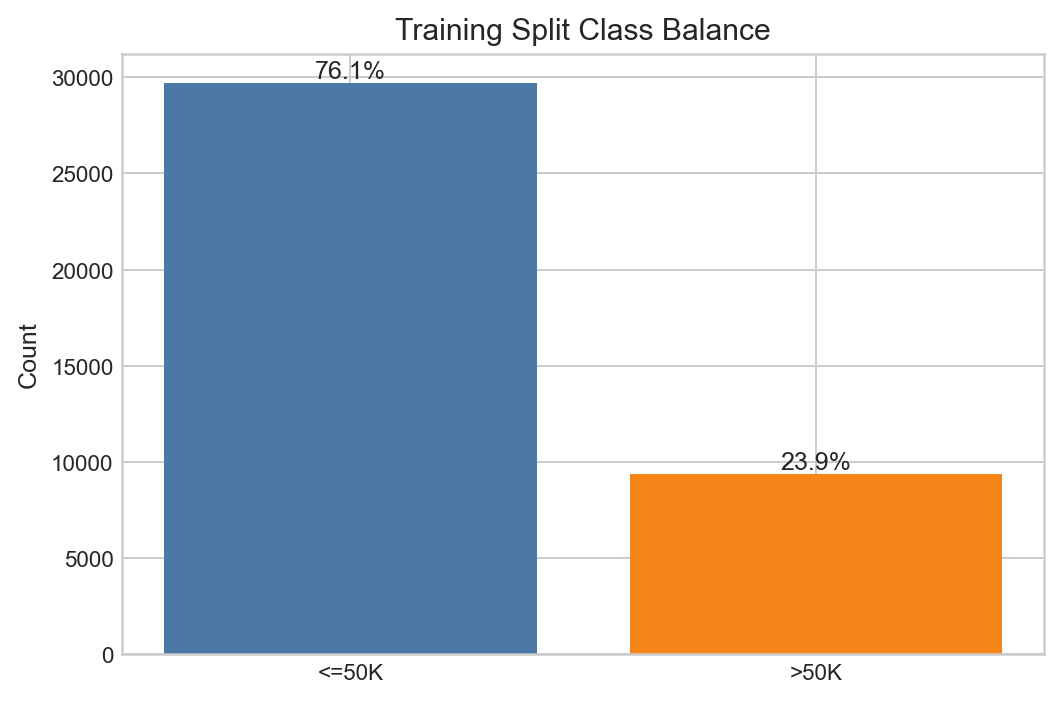
\includegraphics[width=0.88\columnwidth]{figures/class_balance}
  \caption{Class distribution in the training split.  The
    \texttt{>50K} class constitutes 23.9\% of training
    instances, which motivates reporting ROC-AUC alongside
    threshold-dependent metrics.}
  \label{fig:classbalance}
\end{figure}

The continuous features show several patterns that matter for interpretation. \texttt{capital\_gain} is highly sparse, with 91.8\% zeros, and \texttt{capital\_loss} is even sparser, with 95.2\% zeros. \texttt{hours\_per\_week} also has a strong repeated value, with 46.5\% of rows taking one value. These patterns explain why the WhiskerFlow log1p transforms are useful, and they also shape how we interpret the KittenGauss fits. Figure~\ref{fig:continuous} shows visible class separation in \texttt{education\_num} and \texttt{age}, in contrast to the zero-dominated capital variables.

\begin{figure*}[!htb]
  \centering
  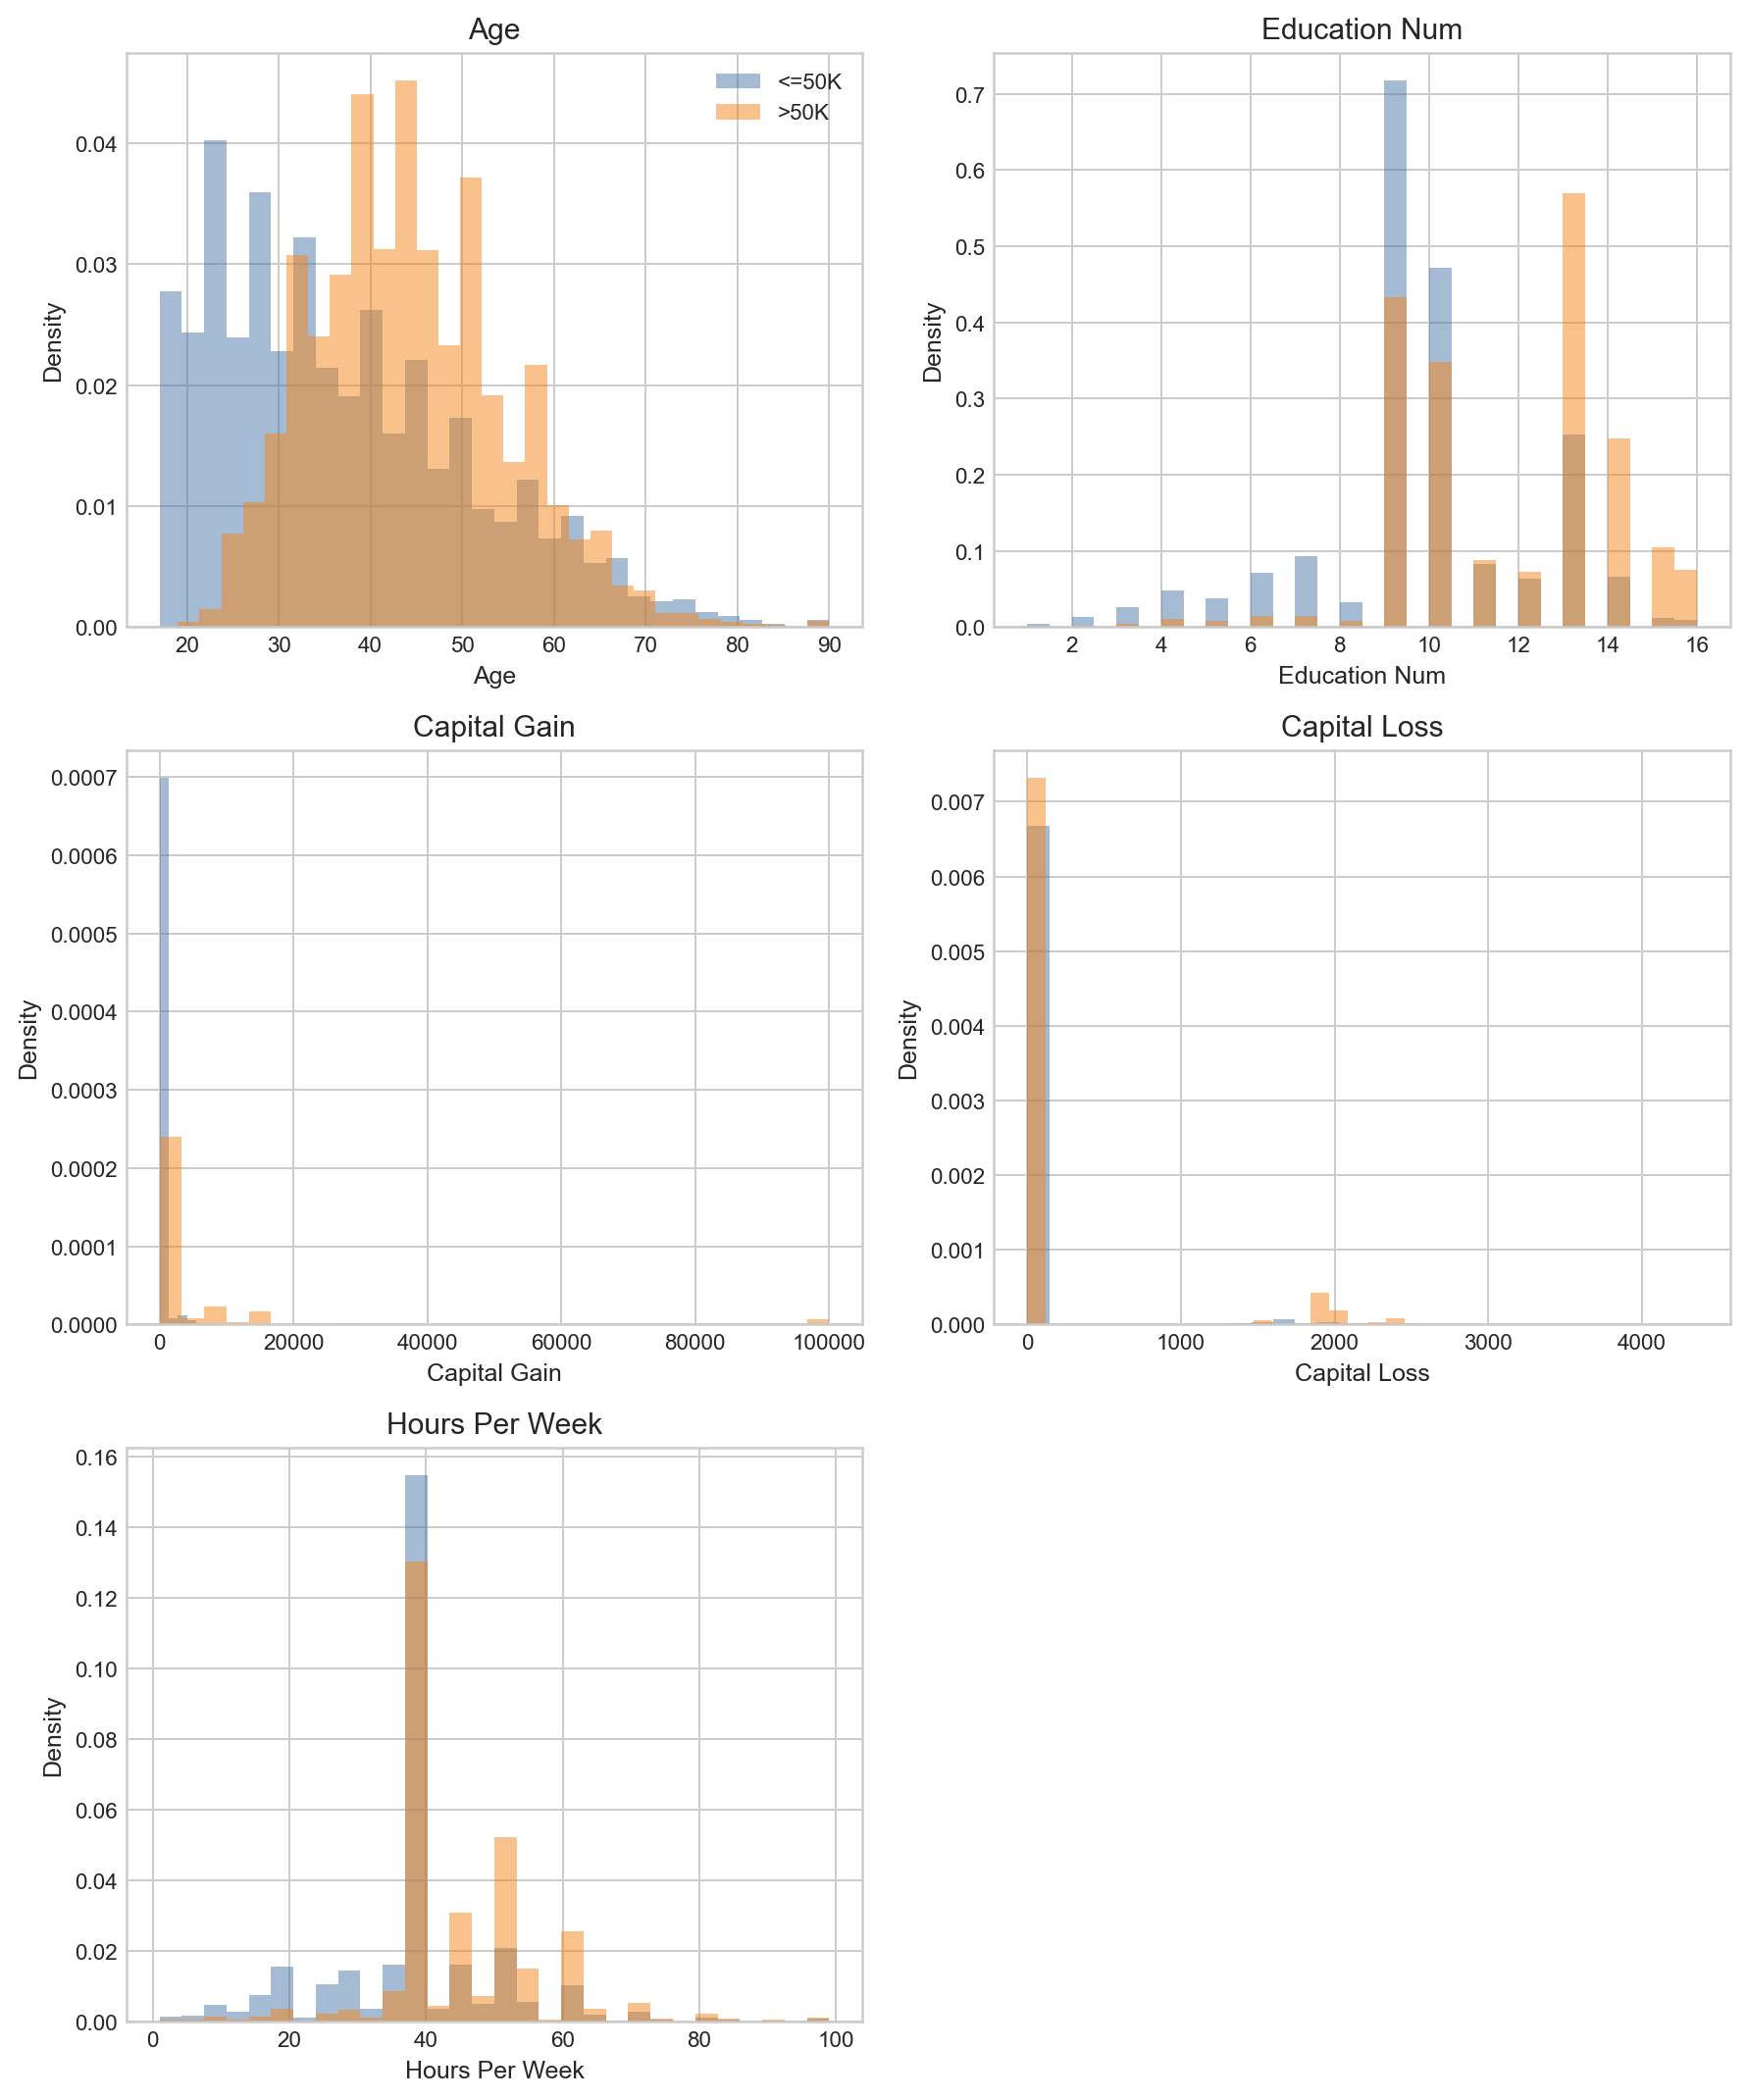
\includegraphics[width=\textwidth]{figures/continuous_by_income_grid}
  \caption{Continuous feature distributions by income class.
    \texttt{education\_num}, \texttt{age}, and
    \texttt{hours\_per\_week} show visible class separation.
    \texttt{capital\_gain} and \texttt{capital\_loss} are dominated
    by a zero mass and long right tails, so a Gaussian summary
    captures their shape poorly.}
  \label{fig:continuous}
\end{figure*}

The categorical variables also show large differences in positive-income rates across groups. Figure~\ref{fig:catfreq} highlights three examples: \texttt{Married-civ-spouse} has a 44.8\% positive rate compared with 4.4\% for \texttt{Never-married}; \texttt{Exec-managerial} has 48.2\% compared with 4.0\% for \texttt{Other-service}; and \texttt{Male} has 30.4\% compared with 10.9\% for \texttt{Female}. These contrasts suggest, before formal modelling, that household structure and occupation-related variables will carry substantial information about the label.

\begin{figure}[!ht]
  \centering
  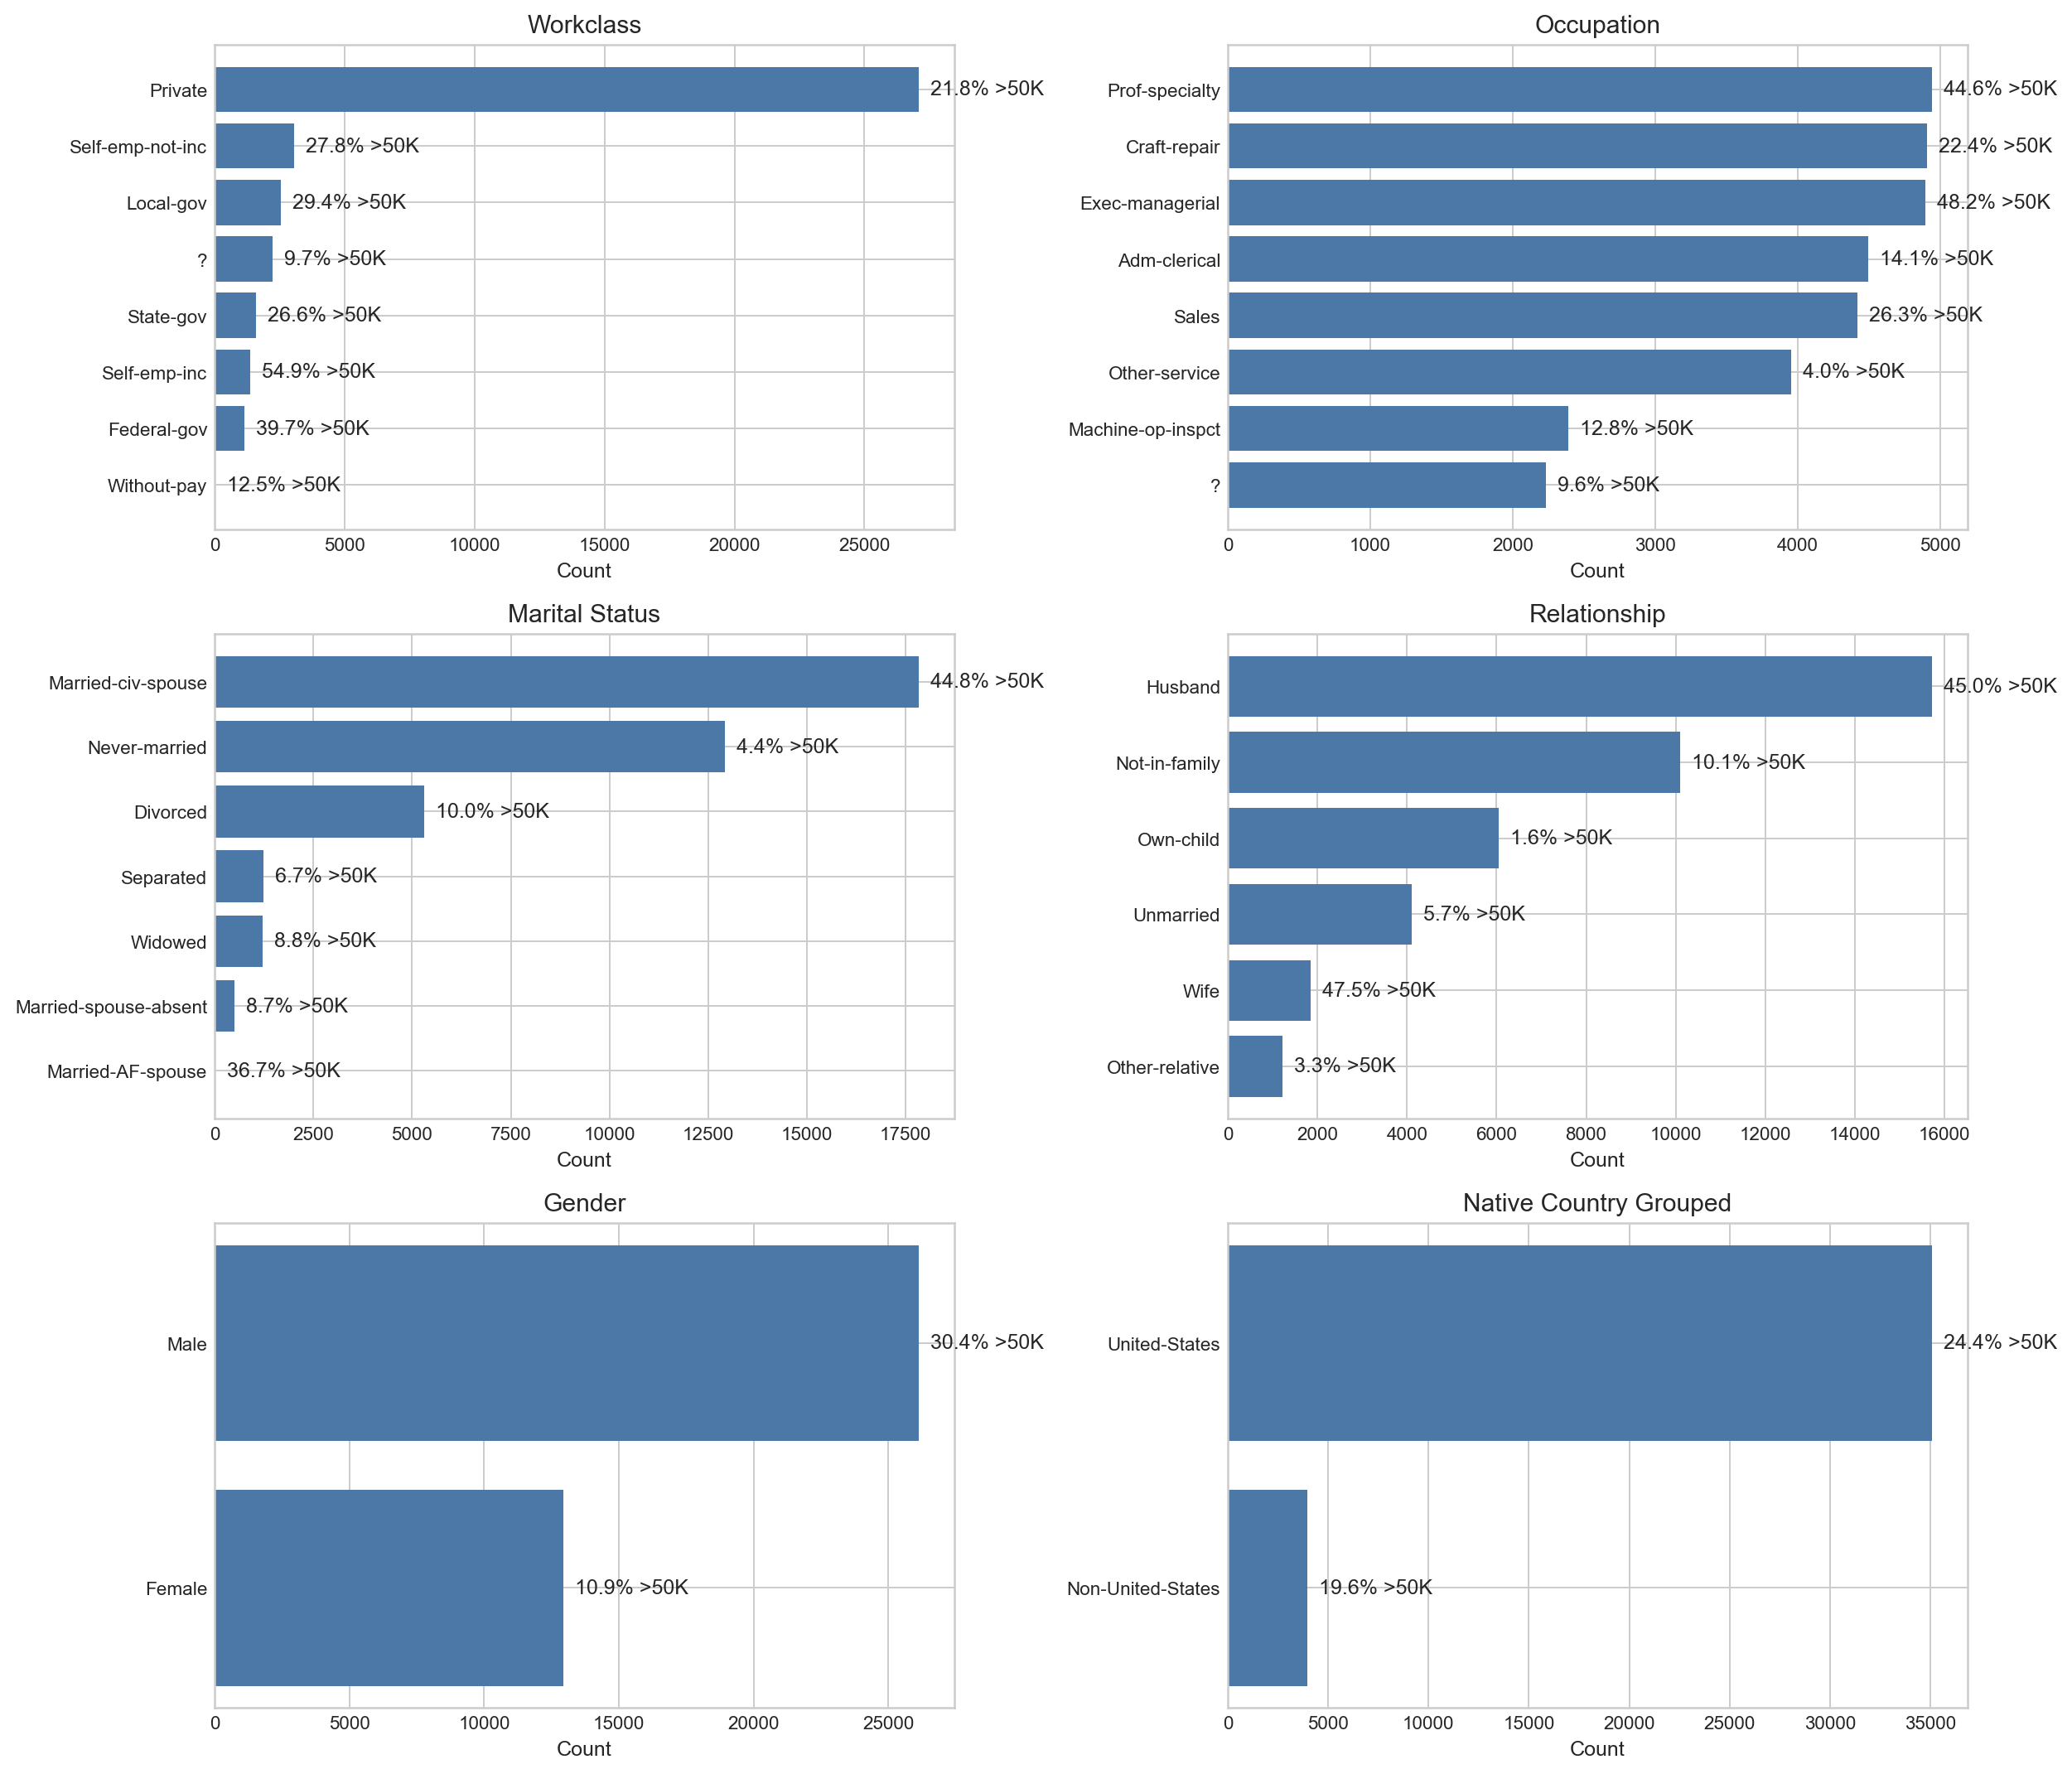
\includegraphics[width=\columnwidth]{figures/categorical_frequency_grid}
  \caption{Selected categorical feature distributions with
    positive-income rates.  Household-structure variables
    (\texttt{marital\_status}, \texttt{relationship}) and
    occupation-related variables show large income-class
    differences before formal modelling.}
  \label{fig:catfreq}
\end{figure}

% ---------------------------------------------------------------
\subsection{KittenGauss Distribution Analysis}
\label{sec:kittengauss_results}
% ---------------------------------------------------------------

Table~\ref{tab:gaussian} reports the class-conditional Gaussian statistics and MeowRank scores for the five continuous features. \texttt{education\_num} has the largest continuous separation under this single-feature view, with a MeowRank ROC-AUC of 0.716 and a Cohen's $d$ of 0.825. \texttt{age} and \texttt{hours\_per\_week} show more moderate separation. The capital variables have identical class medians of zero, which is consistent with their extreme zero inflation.

\begin{table*}[!htb]
  \centering
  \small
  \begin{tabular}{lrrcc}
    \toprule
    \textbf{Feature} &
    \textbf{Mean} (${\leq}$50K) &
    \textbf{Mean} ($>$50K) &
    \textbf{Cohen's~$d$} &
    \textbf{MeowRank AUC} \\
    \midrule
    \texttt{education\_num}   & 9.60  & 11.60 & 0.825 & 0.716 \\
    \texttt{age}              & 36.92 & 44.35 & 0.556 & 0.682 \\
    \texttt{hours\_per\_week} & 38.89 & 45.43 & 0.541 & 0.671 \\
    \texttt{capital\_gain}    & 147.7 & 3950  & 0.532 & 0.588 \\
    \texttt{capital\_loss}    & 55.3  & 200.0 & 0.358 & 0.535 \\
    \bottomrule
  \end{tabular}
  \caption{KittenGauss statistics for the five continuous features.
    MeowRank AUC is the single-feature held-out ROC-AUC.  The capital
    variables have large mean differences but low MeowRank scores,
    which is consistent with their zero-inflated shape.}
  \label{tab:gaussian}
\end{table*}

Figure~\ref{fig:gaussian} overlays empirical histograms with the fitted class-conditional Gaussian curves. The approximation is reasonable for \texttt{education\_num}, \texttt{age}, and \texttt{hours\_per\_week}. It breaks down for \texttt{capital\_gain} and \texttt{capital\_loss}, where the distribution is mostly zero with a sparse right tail. Figure~\ref{fig:sepranking} ranks the five features by MeowRank score and again places \texttt{education\_num} first among the continuous variables.

\begin{figure*}[!htb]
  \centering
  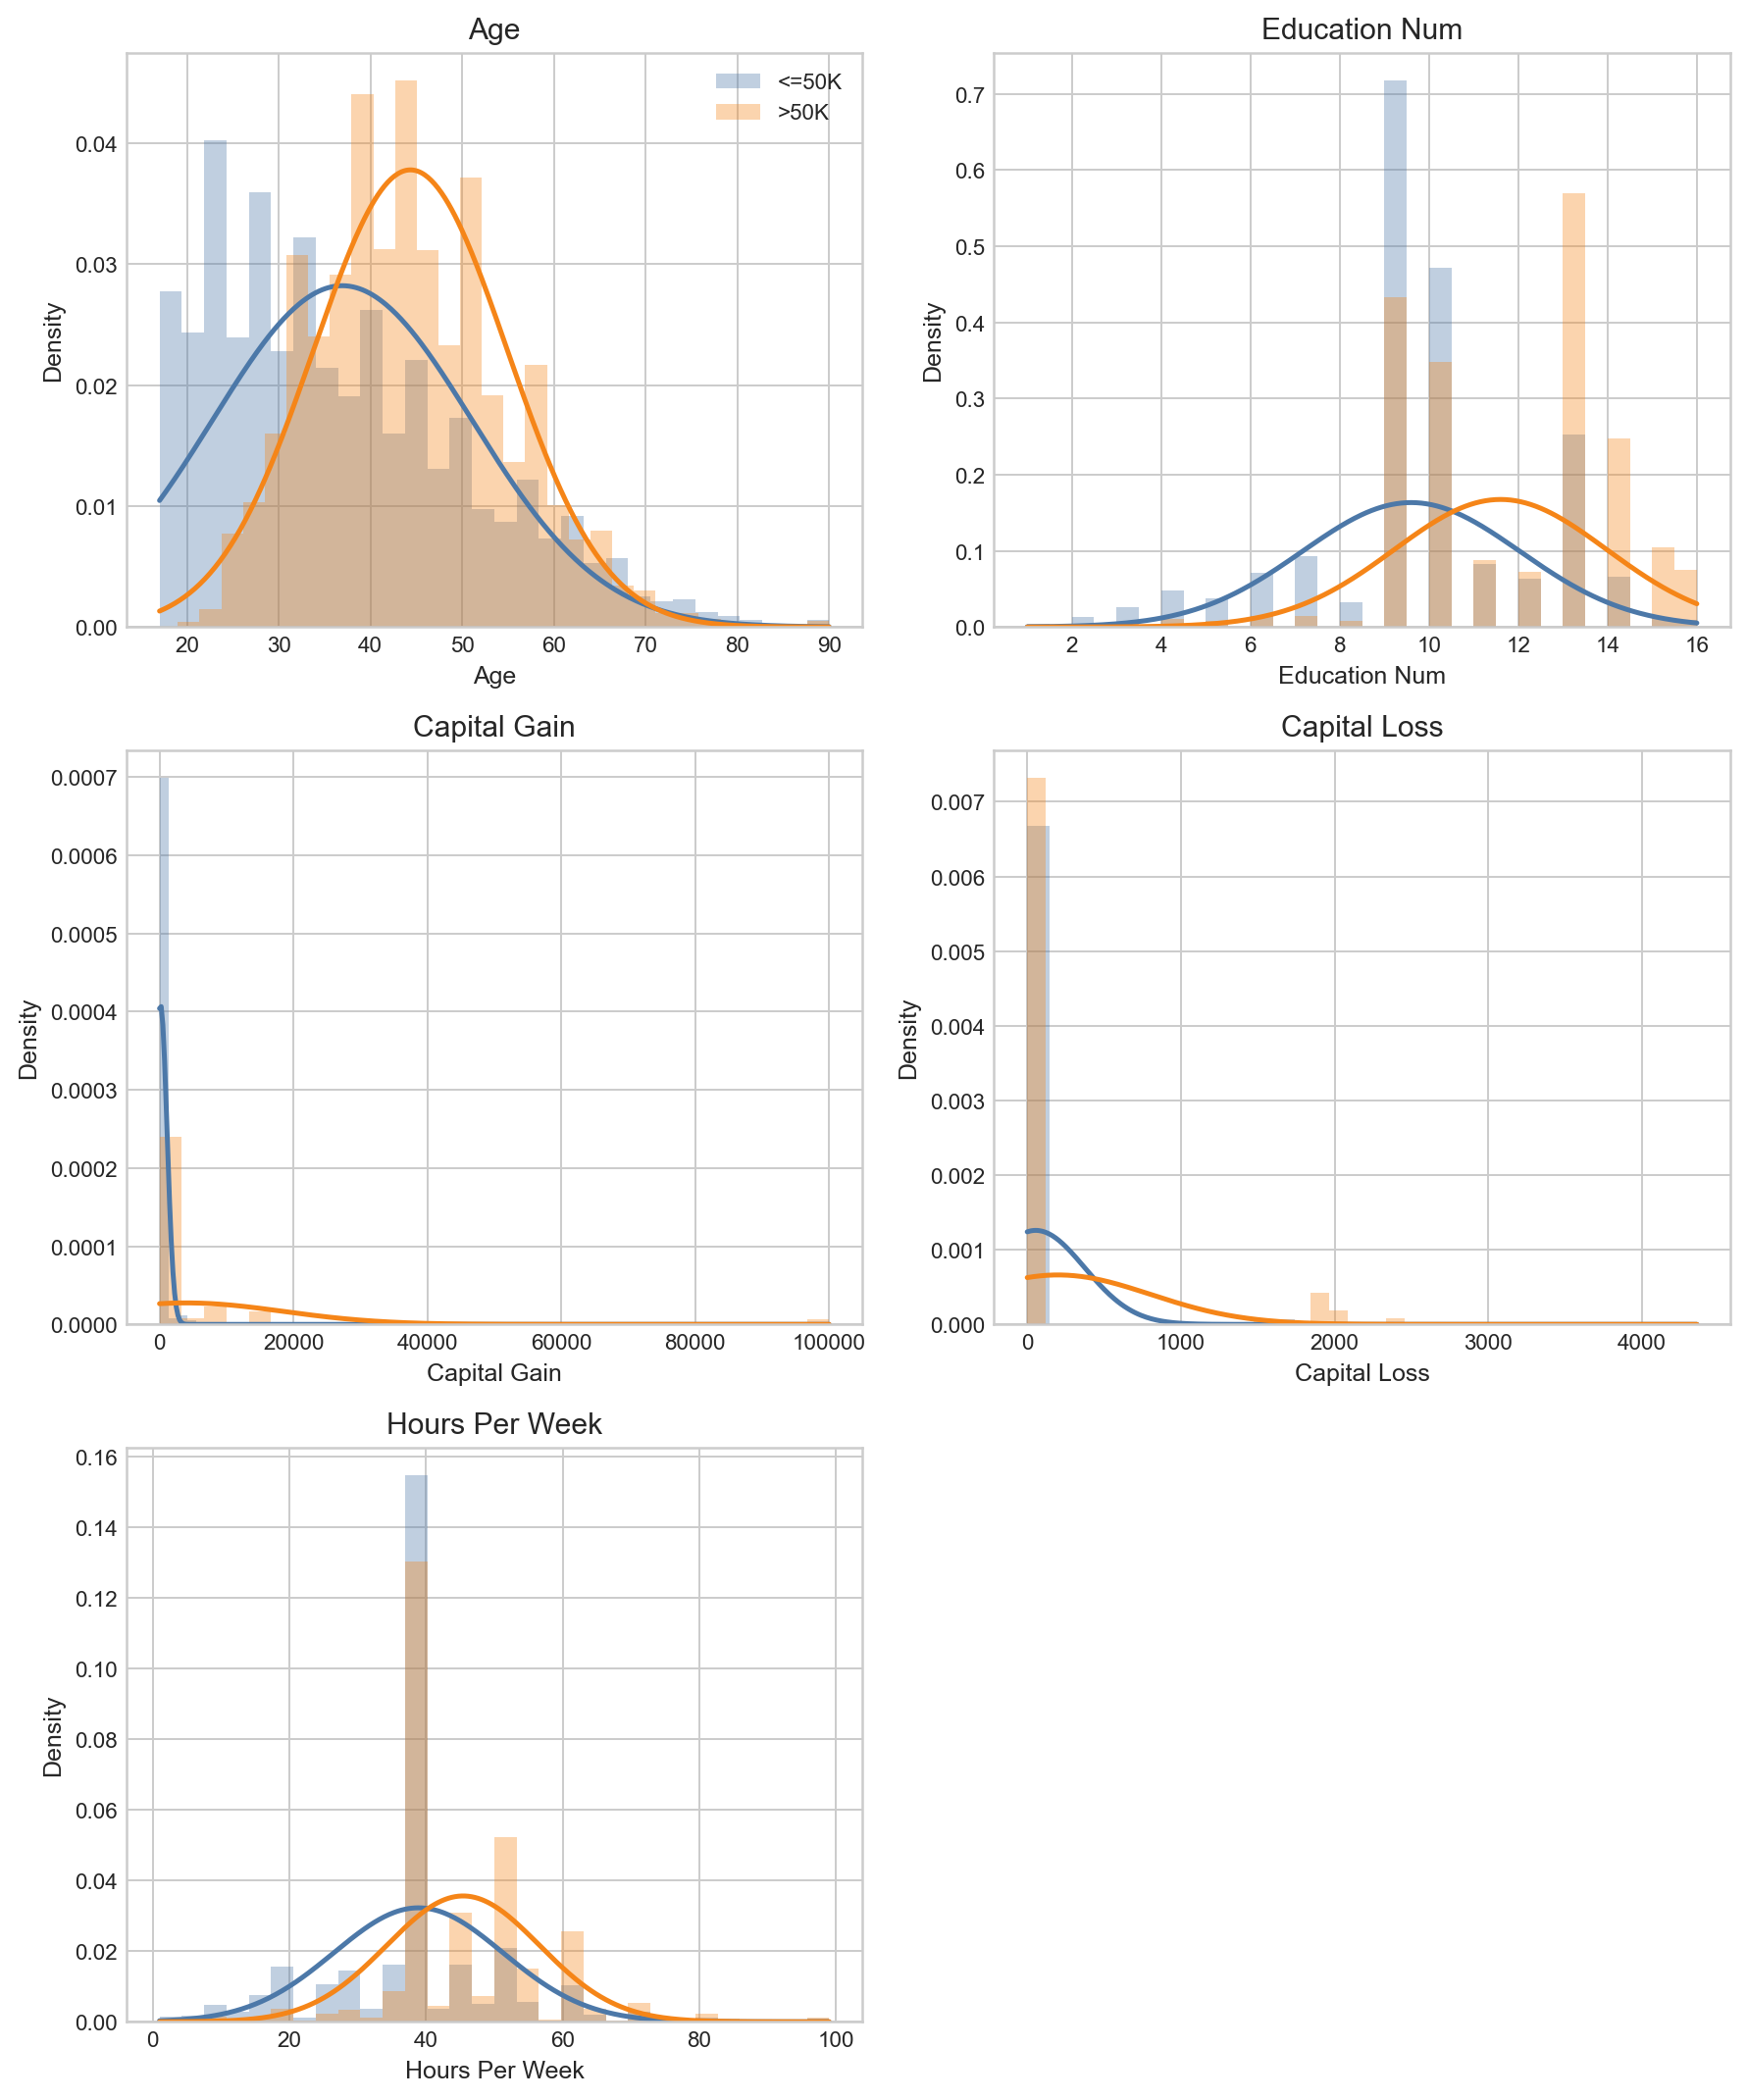
\includegraphics[width=\textwidth]{figures/gaussian_fit_overlays}
  \caption{KittenGauss fitted overlays.  Empirical histograms are
    shown with class-conditional Gaussian curves for each continuous
    feature.  The fit is reasonable for \texttt{education\_num},
    \texttt{age}, and \texttt{hours\_per\_week}, but is a poor
    description of the zero-inflated capital variables.}
  \label{fig:gaussian}
\end{figure*}

\begin{figure}[!ht]
  \centering
  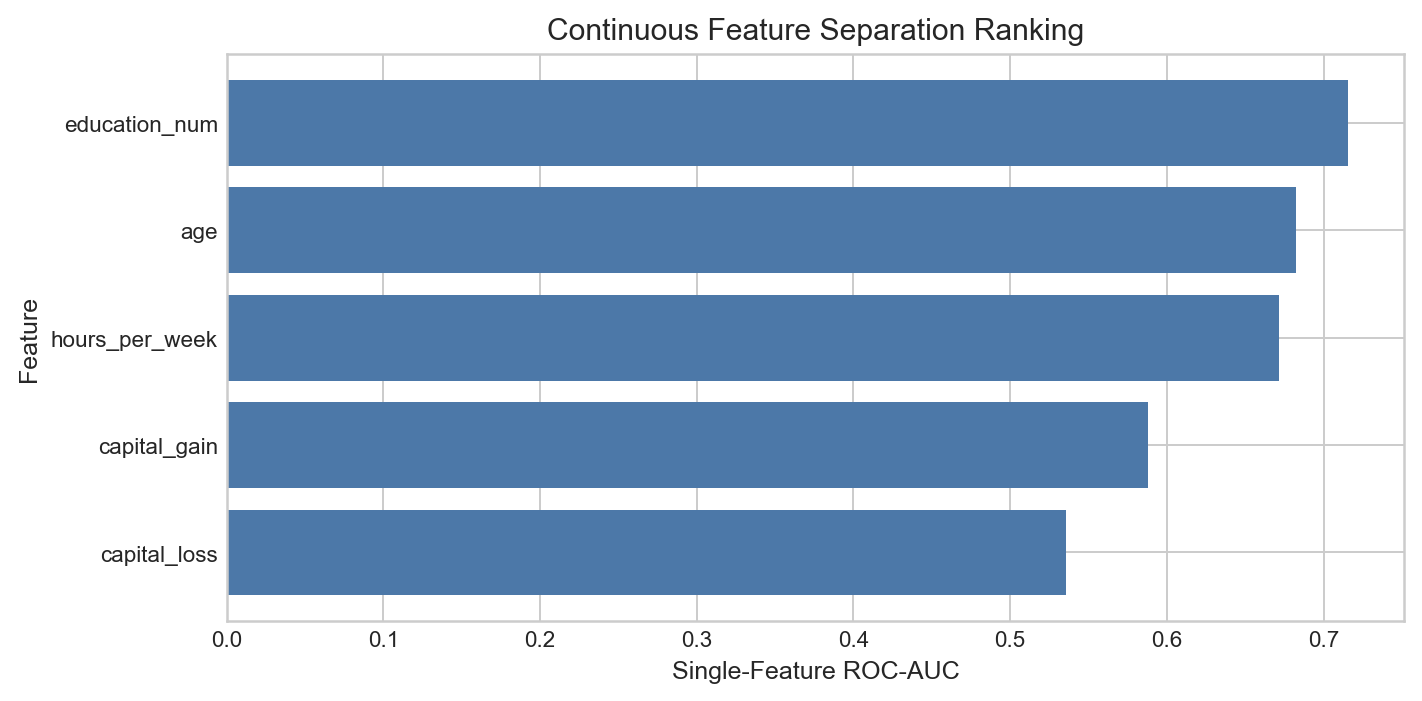
\includegraphics[width=0.92\columnwidth]{figures/continuous_separation_ranking}
  \caption{MeowRank ranking of continuous features by single-feature
    held-out ROC-AUC.  \texttt{education\_num} has the largest
    marginal separation under this metric.}
  \label{fig:sepranking}
\end{figure}

% ---------------------------------------------------------------
\subsection{TailMI Feature Dependencies}
\label{sec:tailmi_results}
% ---------------------------------------------------------------

Table~\ref{tab:tailmi} reports the largest feature--label and feature--feature MI values. The highest feature--label MI values are for \texttt{relationship} (0.116) and \texttt{marital\_status} (0.111). These are above the leading numeric features, including \texttt{age} (0.064) and \texttt{education\_num} (0.062). The largest pairwise dependencies are concentrated among household-structure and work-context variables: \texttt{marital\_status}--\texttt{relationship} ($\hat{I} = 0.725$), \texttt{workclass}--\texttt{occupation} (0.329), and \texttt{relationship}--\texttt{gender} (0.270).

\begin{table}[!ht]
  \centering
  \small
  \begin{tabular}{lc}
    \toprule
    \textbf{Feature} & \textbf{Feature--label MI} \\
    \midrule
    \texttt{relationship}    & 0.116 \\
    \texttt{marital\_status} & 0.111 \\
    \texttt{age}             & 0.064 \\
    \texttt{occupation}      & 0.063 \\
    \texttt{education\_num}  & 0.062 \\
    \texttt{capital\_gain}   & 0.054 \\
    \bottomrule
  \end{tabular}

  \vspace{0.8em}

  \begin{tabular}{lc}
    \toprule
    \textbf{Feature pair} & \textbf{Pairwise MI} \\
    \midrule
    \texttt{marital\_status} $\times$ \texttt{relationship} & 0.725 \\
    \texttt{workclass} $\times$ \texttt{occupation}         & 0.329 \\
    \texttt{relationship} $\times$ \texttt{gender}          & 0.270 \\
    \texttt{age} $\times$ \texttt{marital\_status}          & 0.233 \\
    \texttt{education\_num} $\times$ \texttt{occupation}    & 0.213 \\
    \bottomrule
  \end{tabular}
  \caption{TailMI results.  \textit{Top}: top feature--label MI
    values.  \textit{Bottom}: top five feature--feature MI pairs.
    The high pairwise MI values suggest structural overlap among
    sociodemographic variables.}
  \label{tab:tailmi}
\end{table}

Figure~\ref{fig:miheatmap} shows the full pairwise MI matrix. Figures~\ref{fig:milabel} and~\ref{fig:mipairs} show the feature--label ranking and the leading feature--feature pairs as bar charts. The discretisation sensitivity check gives complete overlap in the top-10 MI pairs (10/10) and in the candidate interaction shortlist (5/5) across the two binning schemes. This suggests that the main TailMI dependency pattern is not an artefact of the chosen bin width.

\begin{figure}[!ht]
  \centering
  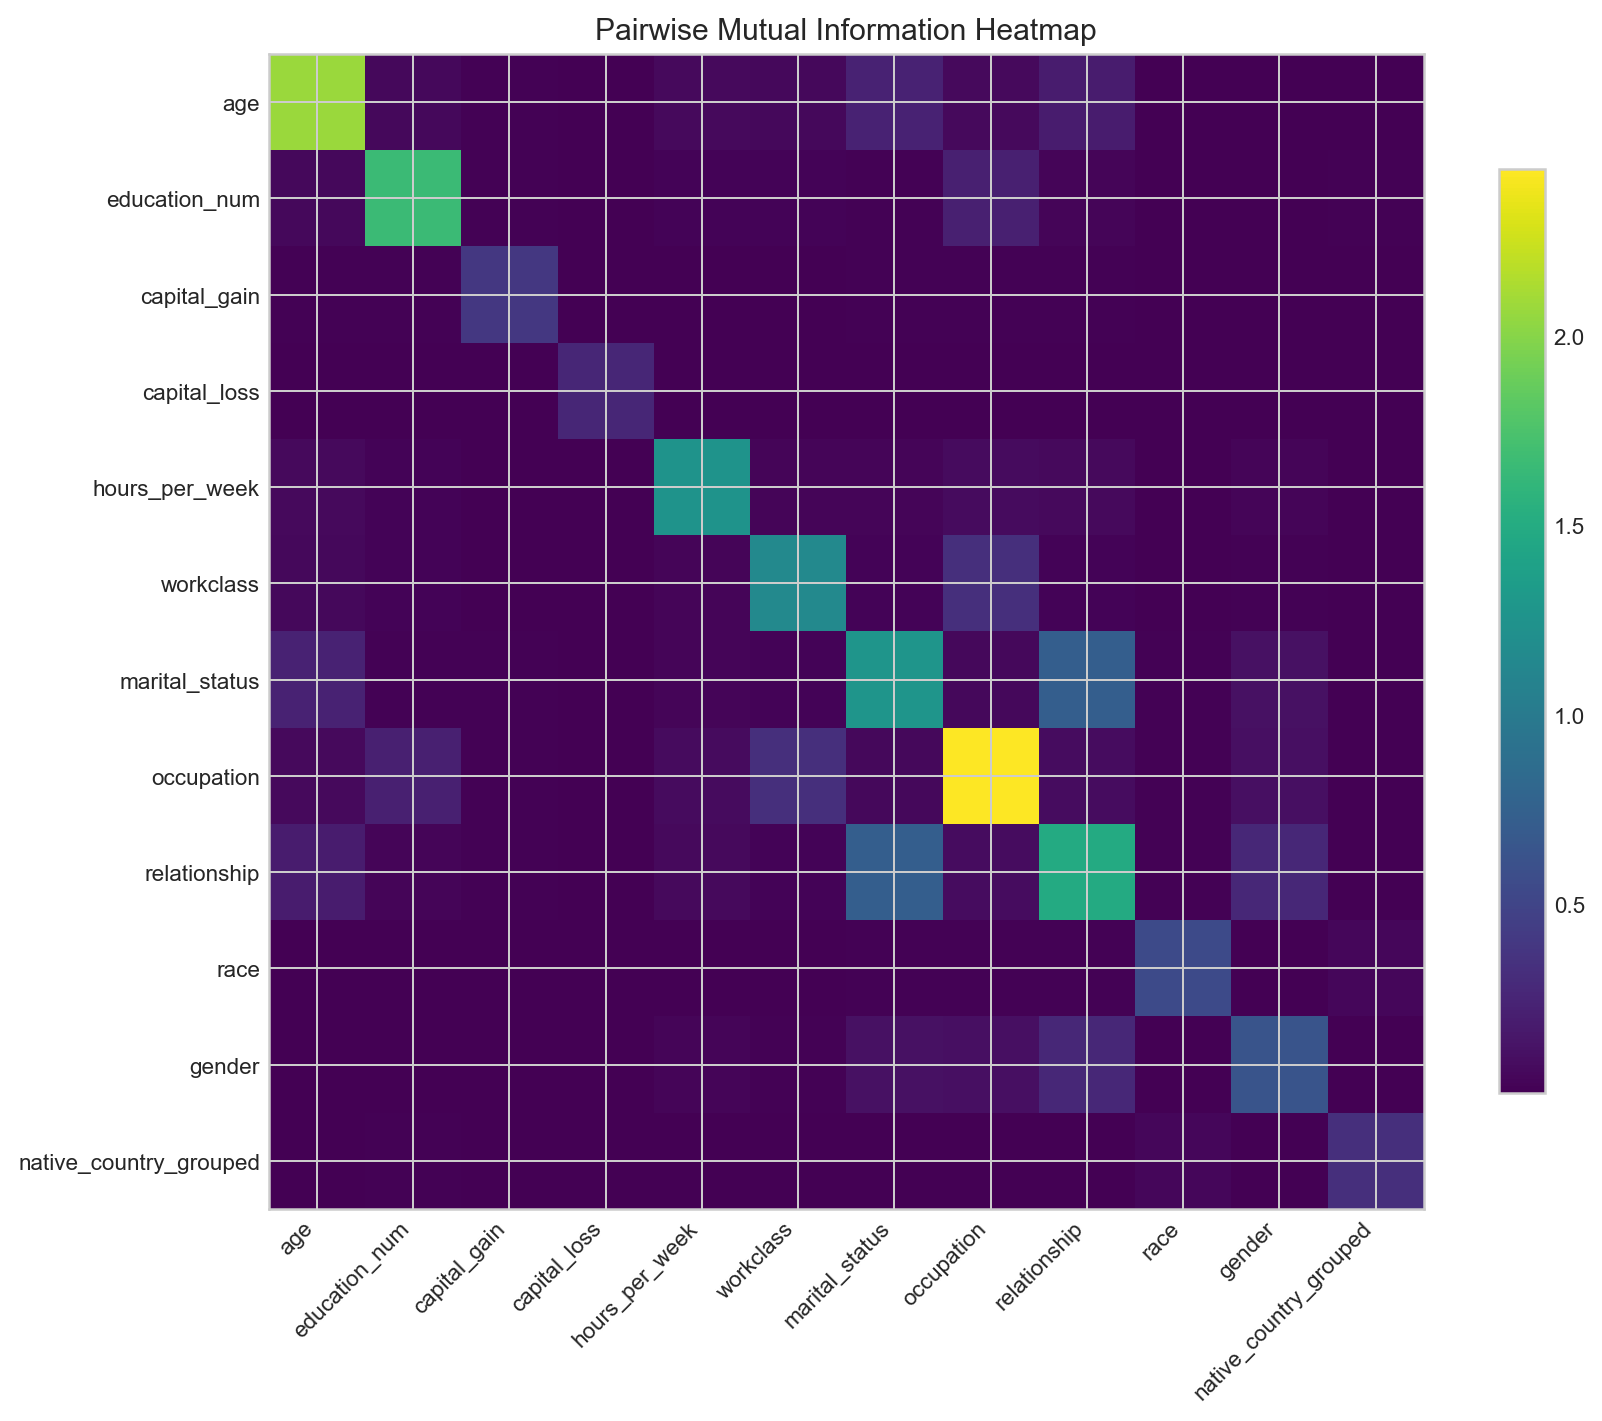
\includegraphics[width=\columnwidth]{figures/mi_heatmap}
  \caption{TailMI pairwise mutual information heatmap.  The largest
    dependencies are concentrated among household-structure and
    work-context variables.  Darker cells indicate higher MI values.}
  \label{fig:miheatmap}
\end{figure}

\begin{figure}[!ht]
  \centering
  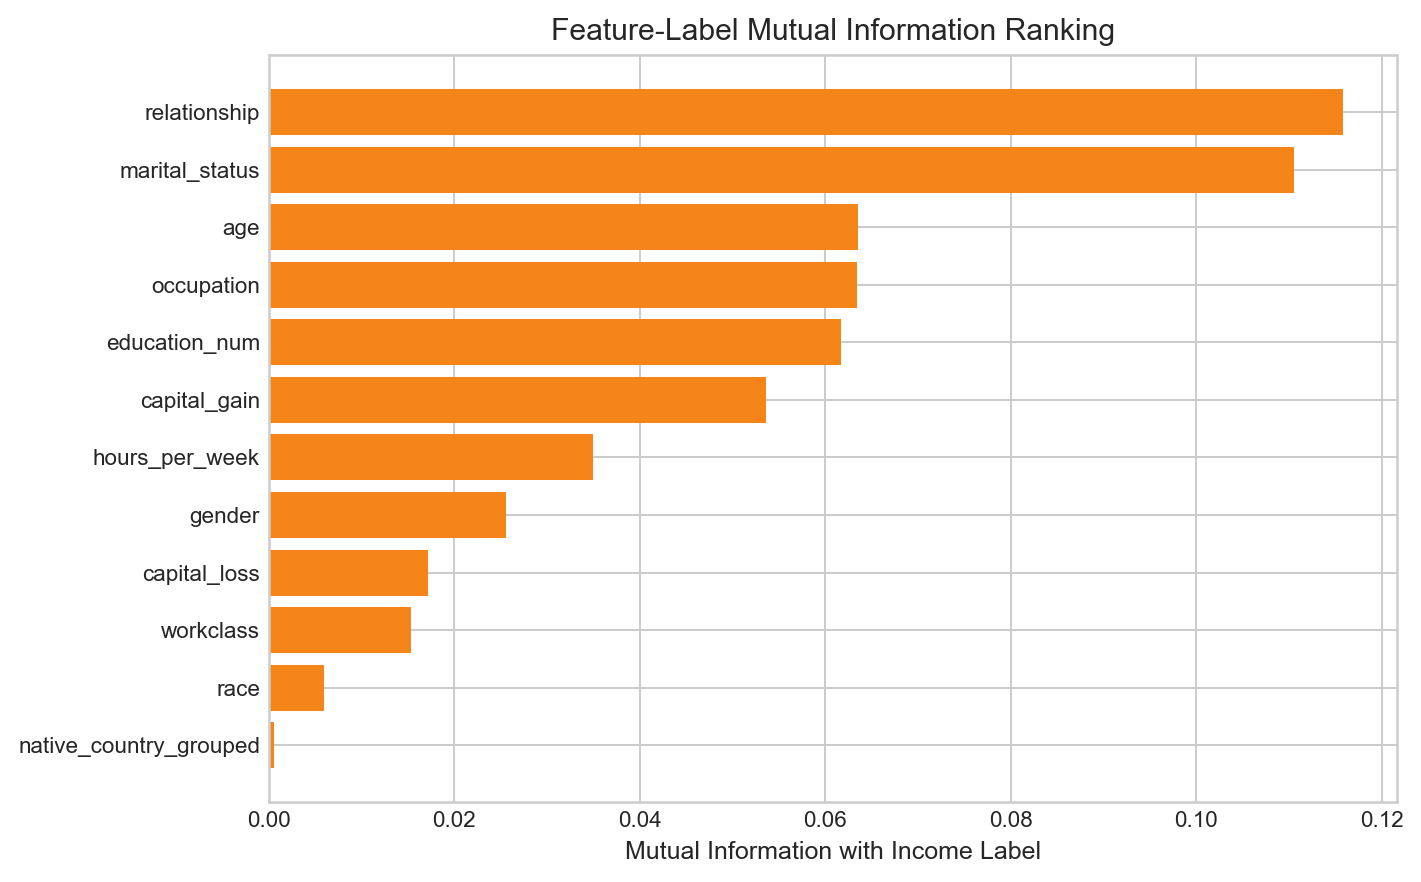
\includegraphics[width=\columnwidth]{figures/feature_label_mi_ranking}
  \caption{TailMI feature--label MI ranking.  \texttt{relationship}
    and \texttt{marital\_status} have the largest marginal MI with
    the income label.}
  \label{fig:milabel}
\end{figure}

\begin{figure}[!ht]
  \centering
  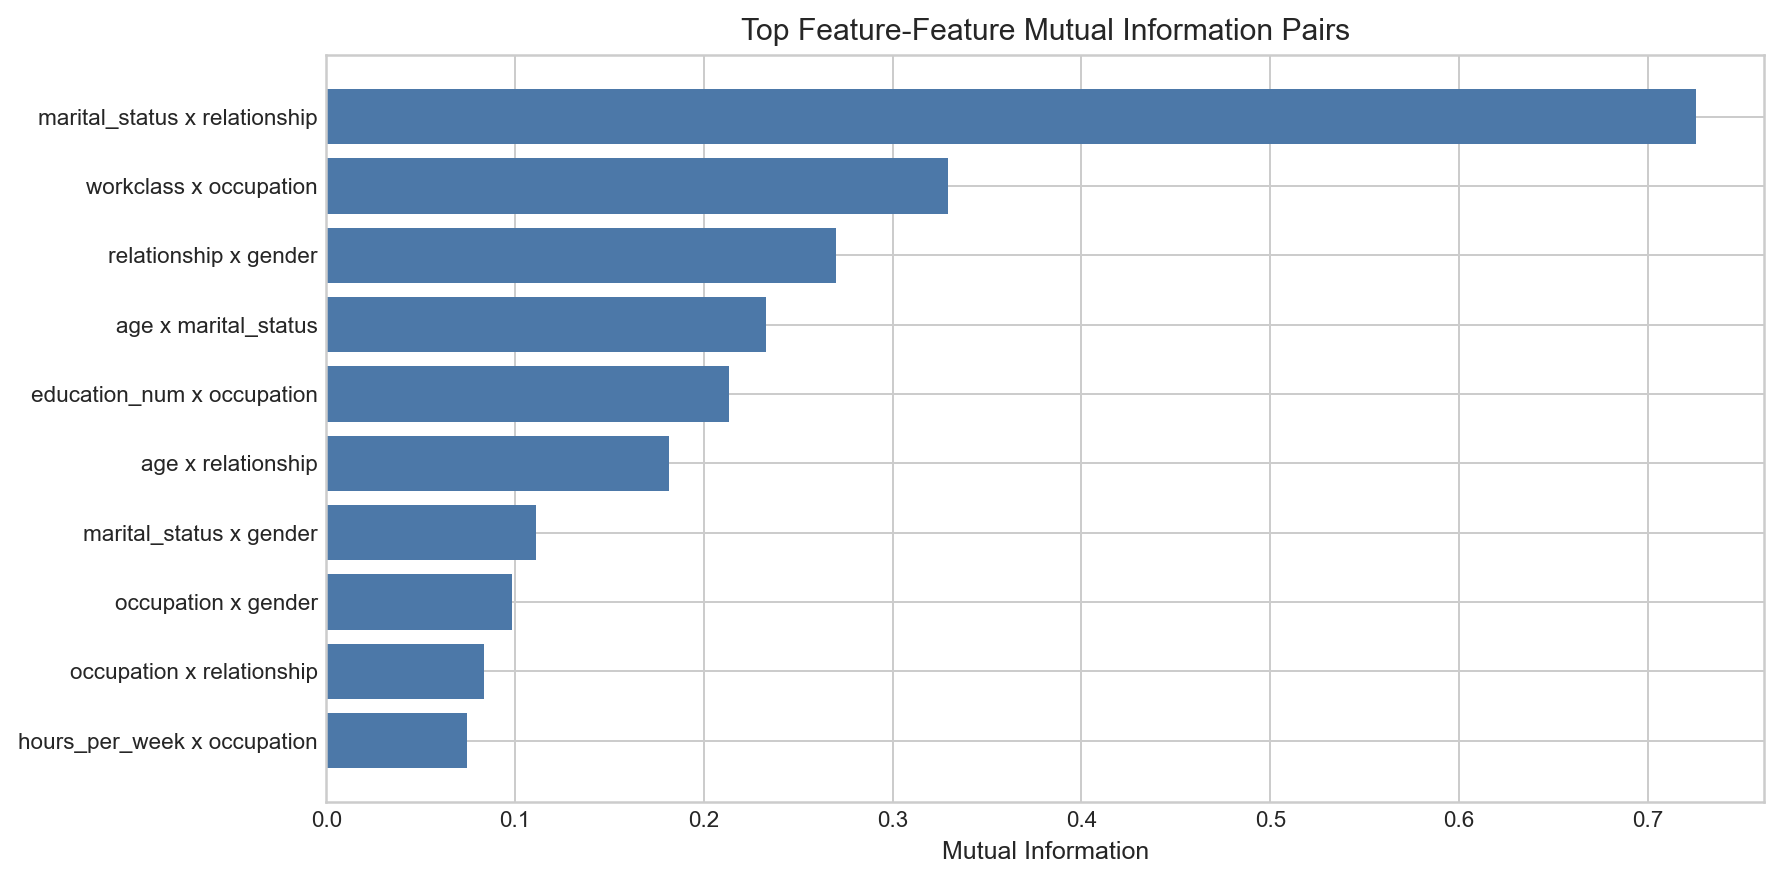
\includegraphics[width=\columnwidth]{figures/top_mi_pairs}
  \caption{Top feature--feature MI pairs.  The largest values mostly
    reflect overlap among sociodemographic variables.}
  \label{fig:mipairs}
\end{figure}

% ---------------------------------------------------------------
\subsection{ClawReg Sparse Model}
\label{sec:clawreg_results}
% ---------------------------------------------------------------

Cross-validation selects $C = 1.0$ for ClawReg. Table~\ref{tab:clawreg} reports the held-out performance of this model, including a test ROC-AUC of 0.897.

\begin{table}[!ht]
  \centering
  \footnotesize
  \begin{tabular}{cccccc}
    \toprule
    \textbf{Acc.} & \textbf{Prec.} & \textbf{Rec.}
      & \textbf{F1} & \textbf{AUC} & \textbf{Best $C$} \\
    \midrule
    0.848 & 0.723 & 0.589 & 0.649 & 0.897 & 1.0 \\
    \bottomrule
  \end{tabular}
  \caption{ClawReg held-out performance on the test split (seed 42).
    Acc.\,=\,accuracy, Prec.\,=\,precision, Rec.\,=\,recall,
    AUC\,=\,ROC-AUC.}
  \label{tab:clawreg}
\end{table}

The cross-validated ROC-AUC rises from 0.887 at $C = 0.001$ to approximately 0.900 by $C = 0.1$. After that point, the curve is nearly flat. From $C = 0.1$ to $C = 10.0$, mean CV ROC-AUC varies by only 0.0003 (0.8998, 0.9001, 0.9001, and 0.9001 at $C = 0.1, 0.316, 1.0, 10.0$). This suggests that the logistic model is not very sensitive to the exact regularisation level once moderate sparsity is allowed.

Table~\ref{tab:stablefeatures} reports feature groups that remain non-zero across the ClawLoss regularisation grid. Six groups are active at all nine grid points: \texttt{marital\_status}, \texttt{education\_num}, \texttt{capital\_gain\_log1p}, \texttt{hours\_per\_week}, \texttt{age}, and \texttt{capital\_loss\_log1p}. Among these, \texttt{marital\_status} has the largest mean absolute coefficient, 3.359, followed by \texttt{education\_num} at 0.741.

\begin{table}[!ht]
  \centering
  \footnotesize
  \setlength{\tabcolsep}{5pt}
  \begin{tabular}{lcc}
    \toprule
    \textbf{Feature group}     & \textbf{Non-zero share} & \textbf{Mean $|\text{coef}|$} \\
    \midrule
    \texttt{marital\_status}       & 1.000 & 3.359 \\
    \texttt{education\_num}        & 1.000 & 0.741 \\
    \texttt{capital\_gain\_log1p}  & 1.000 & 0.475 \\
    \texttt{hours\_per\_week}      & 1.000 & 0.328 \\
    \texttt{age}                   & 1.000 & 0.317 \\
    \texttt{capital\_loss\_log1p}  & 1.000 & 0.220 \\
    \texttt{occupation}            & 0.889 & ---   \\
    \texttt{relationship}          & 0.778 & ---   \\
    \texttt{workclass}             & 0.778 & ---   \\
    \texttt{gender}                & 0.778 & ---   \\
    \bottomrule
  \end{tabular}
  \caption{ClawReg feature group stability across the full
    regularisation grid.  Non-zero share is the fraction of the
    9 grid points at which the group has at least one non-zero
    coefficient.  Groups with non-zero share $< 1$ do not
    appear at all grid points.}
  \label{tab:stablefeatures}
\end{table}

Figure~\ref{fig:coeffpaths} shows the ClawLoss coefficient paths across the regularisation grid. The stable groups remain active across the full path, while several peripheral groups enter only as regularisation weakens. We interpret this as evidence that the model relies on a compact feature core, with additional groups contributing smaller or less stable increments.

\begin{figure*}[!htb]
  \centering
  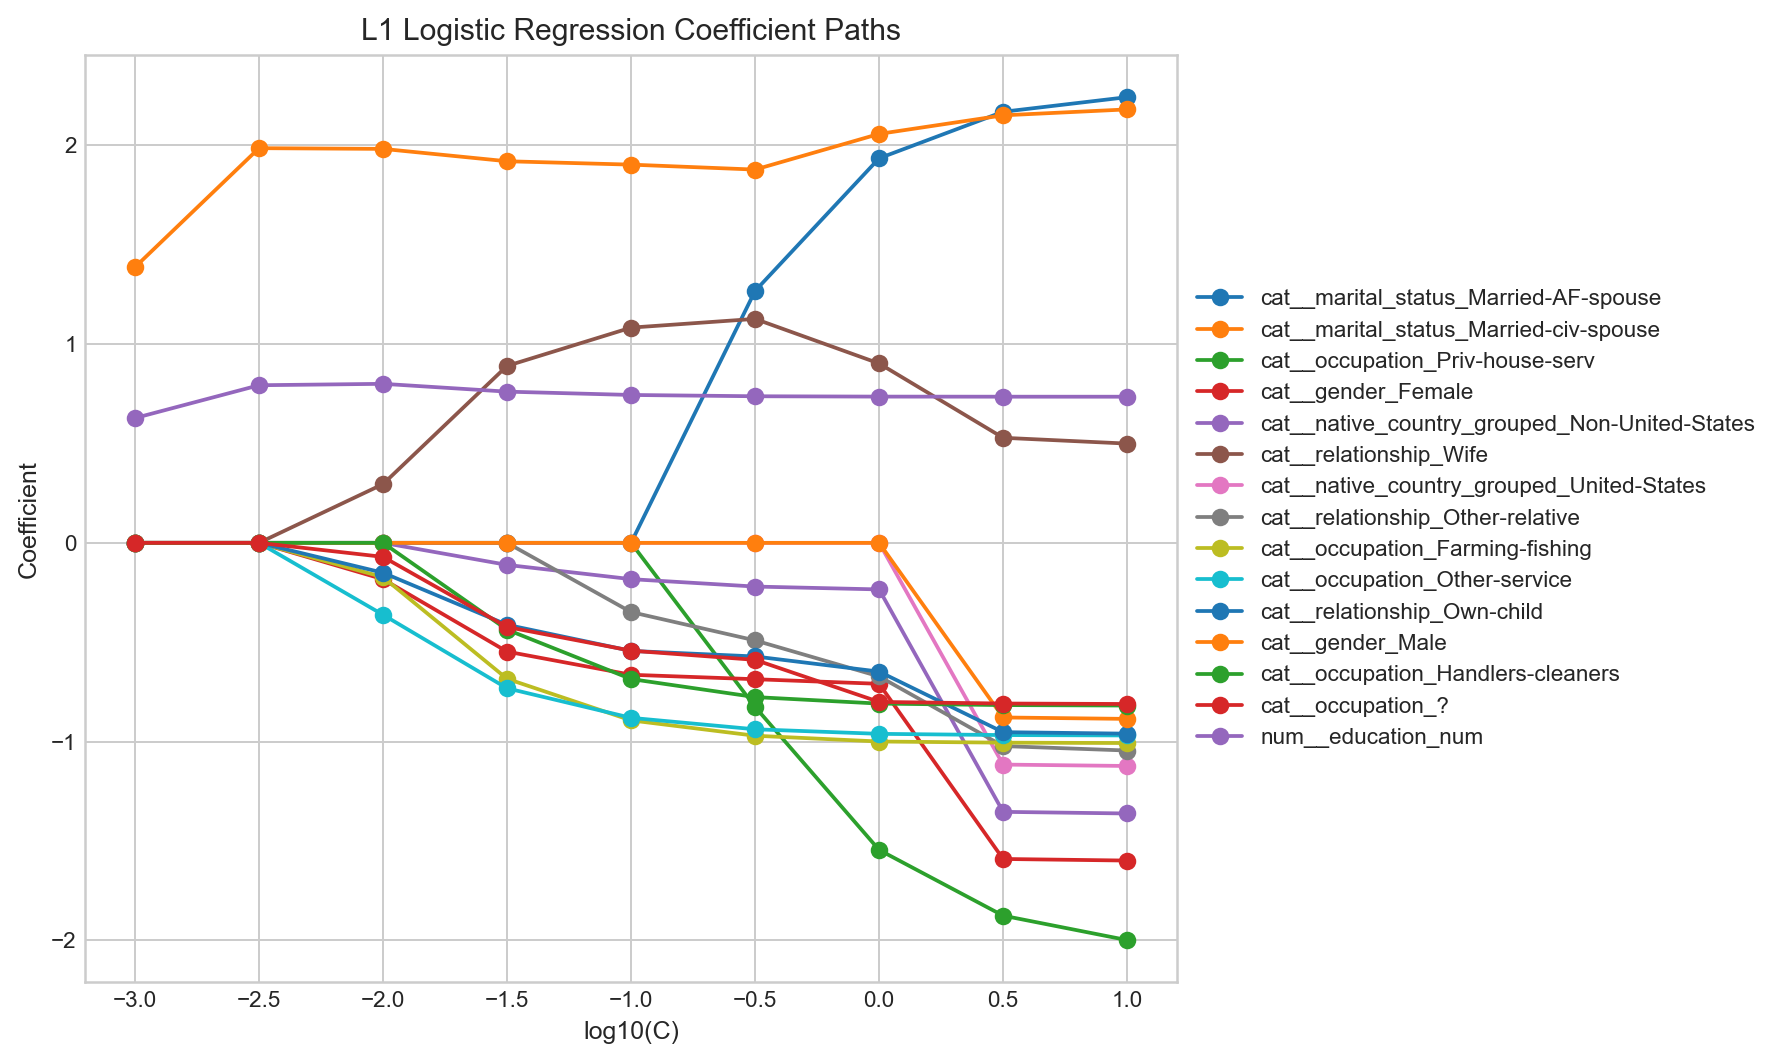
\includegraphics[width=\textwidth]{figures/logistic_coefficient_paths}
  \caption{ClawReg coefficient paths across the L1 regularisation
    grid (ClawLoss).  A compact set of feature groups remains active
    across the full range of regularisation strengths.  The scale of
    the \texttt{marital\_status} coefficient reflects both predictive
    signal and the one-hot encoding of individual categories.}
  \label{fig:coeffpaths}
\end{figure*}

% ---------------------------------------------------------------
\subsection{WhiskerInteract Interaction Validation}
\label{sec:whiskerinteract_results}
% ---------------------------------------------------------------

We next use WhiskerInteract to test five numeric interaction candidates drawn from the TailMI shortlist. Table~\ref{tab:interactions} summarises the results. Every tested interaction changes cross-validated ROC-AUC by less than $10^{-3}$ in magnitude. The largest positive CV change is $+0.000174$ for \texttt{age}~$\times$~\texttt{hours\_per\_week}. None of the tested interactions improves both cross-validation and test ROC-AUC in a consistent way.

\begin{table*}[!htb]
  \centering
  \small
  \begin{tabular}{lccc}
    \toprule
    \textbf{Interaction} &
    \textbf{Pairwise MI} &
    $\boldsymbol{\Delta}$ \textbf{CV AUC} &
    $\boldsymbol{\Delta}$ \textbf{Test AUC} \\
    \midrule
    \texttt{age} $\times$ \texttt{hours\_per\_week}            & 0.066 & $+0.000174$ & $+0.000210$ \\
    \texttt{age} $\times$ \texttt{education\_num}              & 0.052 & $-0.000026$ & $-0.000012$ \\
    \texttt{education\_num} $\times$ \texttt{hours\_per\_week} & 0.027 & $-0.000043$ & $-0.000003$ \\
    \texttt{education\_num} $\times$ \texttt{capital\_gain}    & 0.016 & $-0.000025$ & $+0.000057$ \\
    \texttt{capital\_gain} $\times$ \texttt{hours\_per\_week}  & 0.008 & $+0.000042$ & $-0.000066$ \\
    \bottomrule
  \end{tabular}
  \caption{WhiskerInteract results.  All ROC-AUC deltas fall below
    the $0.001$ improvement threshold, so no interaction-augmented
    model was retained.}
  \label{tab:interactions}
\end{table*}

Because no interaction clears the 0.001 threshold, and because the test-set delta signs vary across candidates, we do not retain an interaction-augmented final model. Figure~\ref{fig:interactions} shows the same pattern visually.

\begin{figure}[!ht]
  \centering
  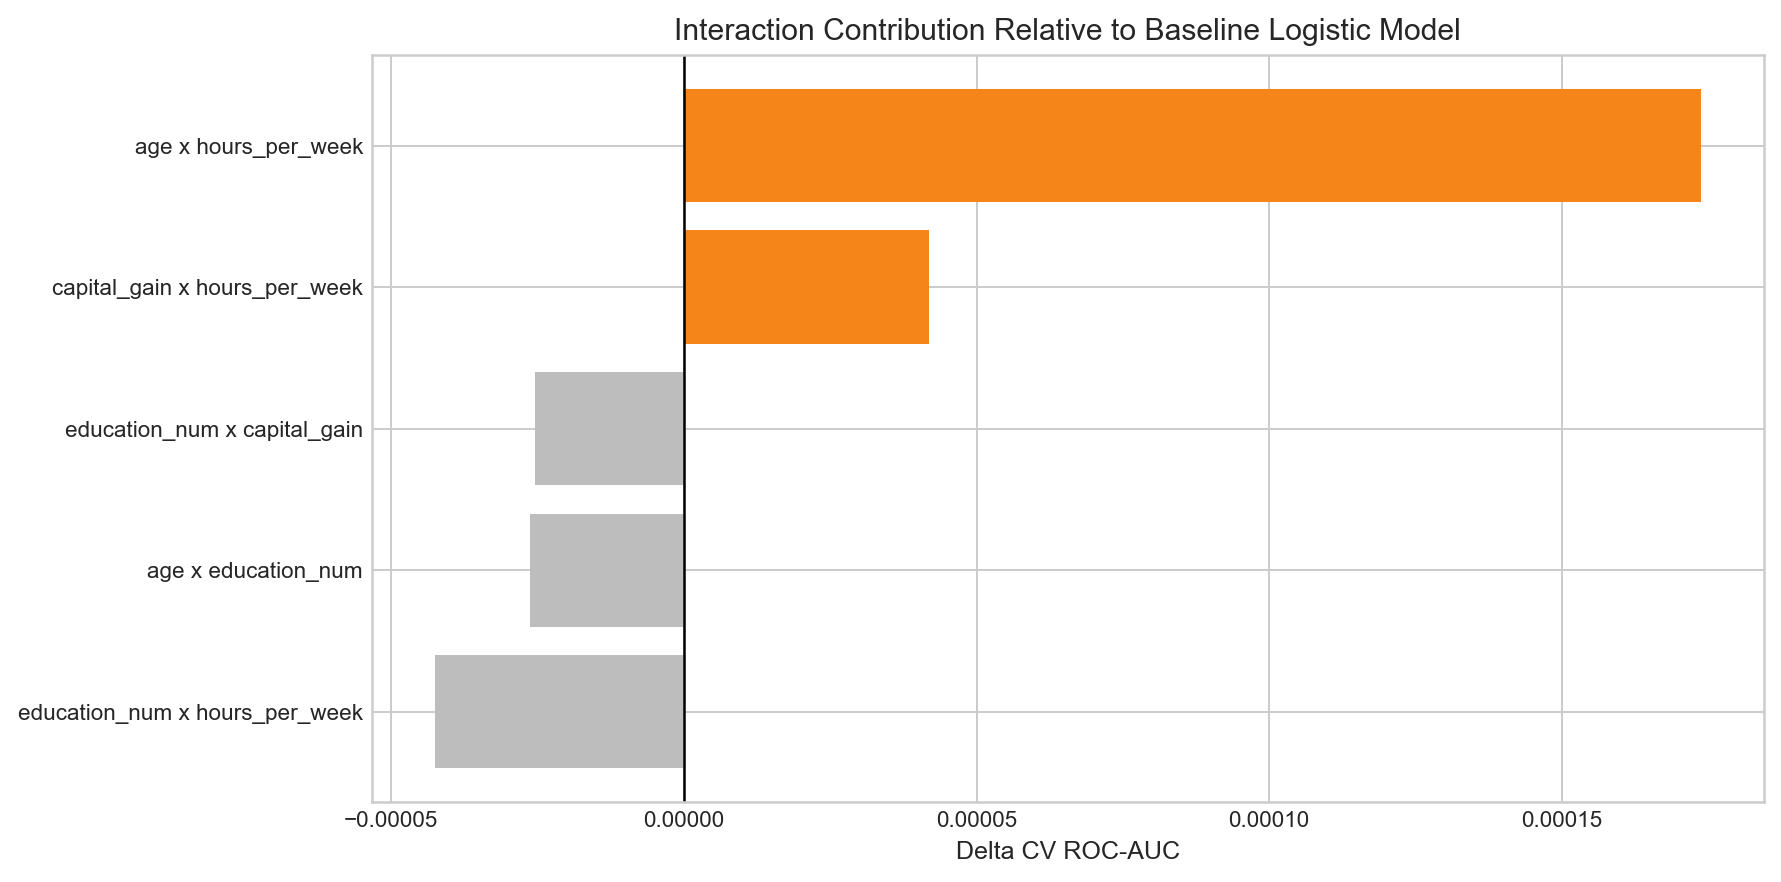
\includegraphics[width=0.9\columnwidth]{figures/interaction_delta_cv_auc}
  \caption{WhiskerInteract: incremental change in CV ROC-AUC from
    adding each interaction term.  All effects are below the
    $0.001$ threshold.}
  \label{fig:interactions}
\end{figure}

% ---------------------------------------------------------------
\subsection{PawSVM Boundary Analysis}
\label{sec:pawsvm_results}
% ---------------------------------------------------------------

Table~\ref{tab:svm} compares the three PawSVM variants. TabbySVM reaches a test ROC-AUC of 0.897 at $C = 0.1$. PurrPoly with degree 2 reaches 0.905, about 0.008 higher. FurRBF reaches 0.896, slightly below TabbySVM.

\begin{table*}[!htb]
  \centering
  \small
  \begin{tabular}{llccc}
    \toprule
    \textbf{Model} & \textbf{Best hyperparameters} &
      \textbf{CV AUC} & \textbf{Test AUC} & \textbf{Test F1} \\
    \midrule
    TabbySVM (linear) & $C = 0.1$                          & 0.893 & 0.897 & 0.644 \\
    PurrPoly (poly-2) & $d=2,\ C=1.0,\ r=1.0$             & 0.898 & 0.905 & 0.670 \\
    FurRBF (RBF)      & $C=3.0,\ \gamma=0.05$             & 0.892 & 0.896 & 0.670 \\
    \bottomrule
  \end{tabular}
  \caption{PawSVM comparison across TabbySVM, PurrPoly, and FurRBF.
    PurrPoly has the highest held-out ROC-AUC.  FurRBF does not
    improve over TabbySVM in this setting.}
  \label{tab:svm}
\end{table*}

The degree-3 PurrPoly variant performs worse in cross-validation (CV ROC-AUC $\approx 0.883$) than degree 2 (0.898). This suggests that the useful nonlinear signal is low-order. The FurRBF result is also consistent with the WhiskerInteract results: the dataset does not appear to require a highly flexible local boundary. One possible explanation for the PurrPoly gain is that the degree-2 kernel captures many small second-order effects across the full encoded feature space, rather than a small set of large numeric products. Figure~\ref{fig:svm} summarises the held-out ROC-AUC comparison.

\begin{figure}[!ht]
  \centering
  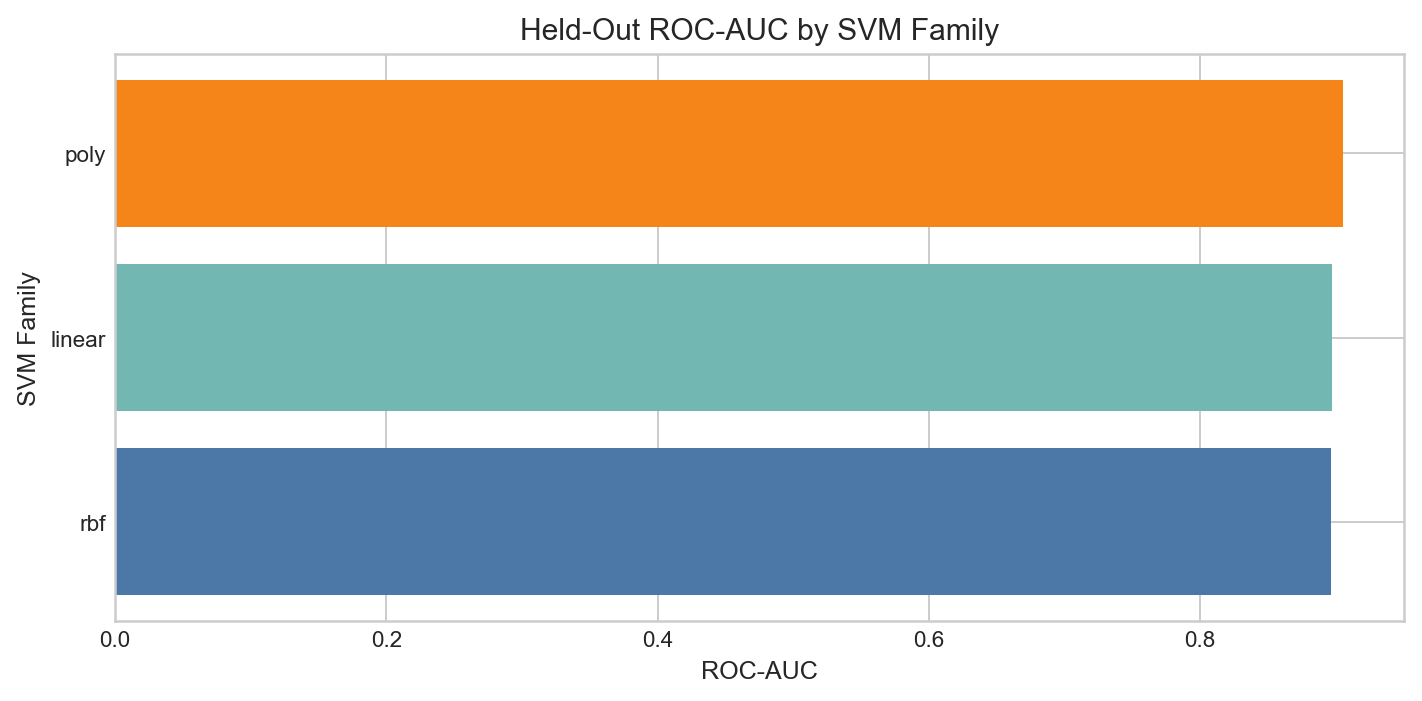
\includegraphics[width=0.9\columnwidth]{figures/svm_kernel_comparison}
  \caption{PawSVM held-out ROC-AUC comparison.  PurrPoly (degree-2
    polynomial) has the highest ROC-AUC among the tested kernels, suggesting
    modest low-order nonlinearity.}
  \label{fig:svm}
\end{figure}

% ---------------------------------------------------------------
\subsection{PurrRobust Stability Checks}
\label{sec:purrobust}
% ---------------------------------------------------------------

Table~\ref{tab:robustness} reports held-out test ROC-AUC for the three main models across random seeds 7, 42, and 99. The ranges are narrow: ClawReg spans 0.897--0.901, TabbySVM spans 0.897--0.901, and PurrPoly spans 0.905--0.906. PurrPoly remains above TabbySVM at every seed, with margins of $+0.0063$, $+0.0078$, and $+0.0045$ at seeds 7, 42, and 99, respectively.

\begin{table}[!ht]
  \centering
  \small
  \begin{tabular}{lcccc}
    \toprule
    \textbf{Model} & \textbf{Seed 7} & \textbf{Seed 42} & \textbf{Seed 99} & \textbf{Range} \\
    \midrule
    ClawReg   & 0.901 & 0.897 & 0.901 & 0.004 \\
    TabbySVM  & 0.900 & 0.897 & 0.901 & 0.004 \\
    PurrPoly  & 0.906 & 0.905 & 0.906 & 0.001 \\
    \bottomrule
  \end{tabular}
  \caption{PurrRobust seed stability.  Held-out test ROC-AUC across
    three stratified random splits.  PurrPoly leads at every seed,
    and all models show narrow variation across splits.}
  \label{tab:robustness}
\end{table}

The TailMI discretisation sensitivity check points in the same direction. The top-10 MI pairs have complete overlap (10/10) across the two binning schemes, and the candidate interaction shortlist also has complete overlap (5/5). Figure~\ref{fig:robustness} shows the metric ranges across seeds.

\begin{figure}[!ht]
  \centering
  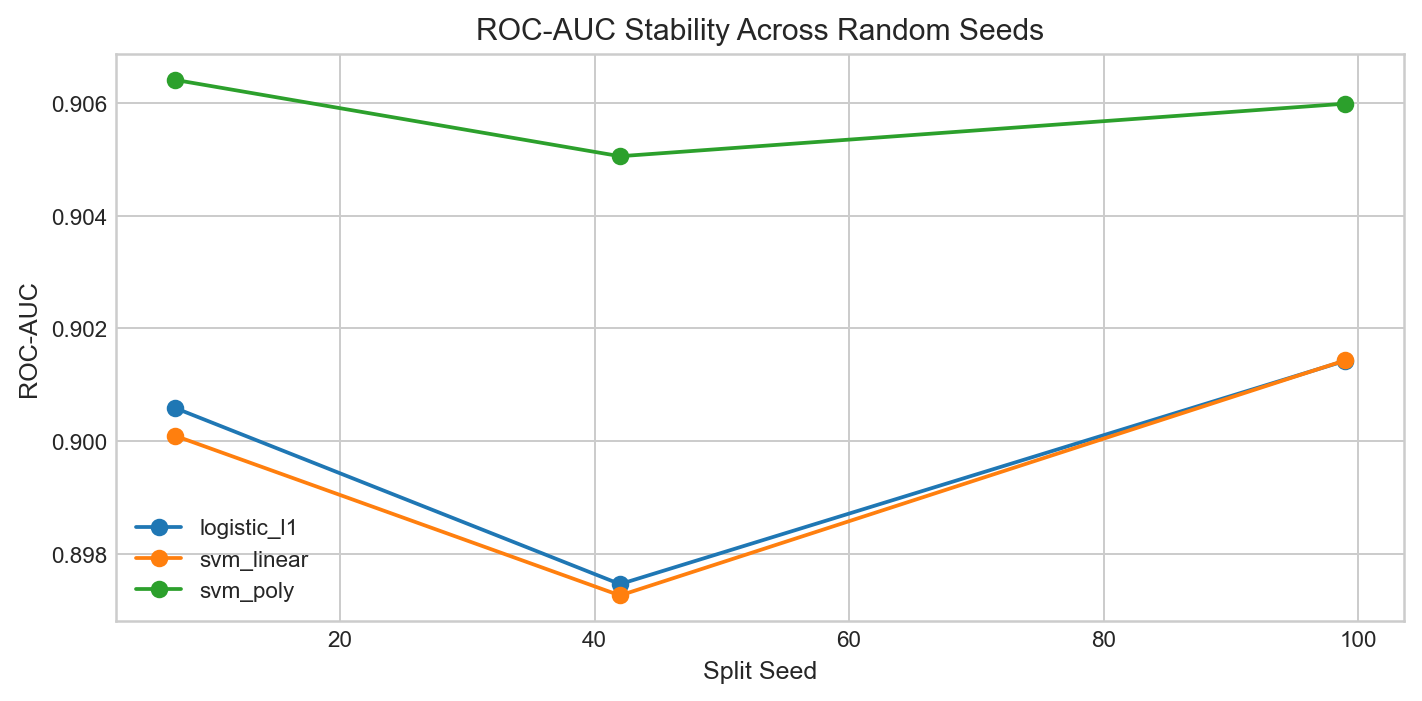
\includegraphics[width=0.9\columnwidth]{figures/robustness_metric_ranges}
  \caption{PurrRobust: ROC-AUC metric ranges across seeds 7, 42,
    and 99.  The ordering of PurrPoly above TabbySVM and ClawReg
    is stable across the three splits.}
  \label{fig:robustness}
\end{figure}

% ===============================================================
\section{Evaluation Metrics Used}
\label{sec:evaluation}
% ===============================================================

Taken together, the six CatNet modules give a consistent picture of the Adult income dataset. The clearest signals come from household-structure and education-related variables. This pattern appears in the TailMI feature--label ranking, the KittenGauss MeowRank scores, and the ClawReg stability analysis. We interpret this cross-method agreement as useful evidence because the methods make different assumptions and fail in different ways.

The comparison between TailMI and ClawReg adds an important qualification. \texttt{relationship} has the highest feature--label MI (0.116), but it is less stable in ClawReg than \texttt{marital\_status}, whose feature--label MI is 0.111. One possible explanation is that the two variables encode overlapping information about household role. Once \texttt{marital\_status} is included in the model, \texttt{relationship} contributes less additional signal. This interpretation is consistent with their large pairwise MI of 0.725. The broader implication is that MI rankings should not be read as multivariate feature-importance rankings. High marginal relevance does not necessarily imply low redundancy.

The capital variables illustrate why it helps to compare several views of the same data. Under KittenGauss, \texttt{capital\_gain} and \texttt{capital\_loss} look poorly described by Gaussian summaries, and their single-feature MeowRank scores are low. After the WhiskerFlow log1p transform, however, \texttt{capital\_gain\_log1p} and \texttt{capital\_loss\_log1p} both survive the full ClawReg regularisation path. This suggests that the apparent weakness of these variables is partly a representation issue. A feature can look uninformative under one summary while still mattering after a more suitable transformation.

The PawSVM boundary analysis addresses the fourth research question. The results suggest that the income decision boundary is not purely linear, but that the nonlinearity is modest. Degree-2 PurrPoly improves ROC-AUC over TabbySVM by roughly 0.008 across the tested seeds, while FurRBF does not improve over the linear baseline. This points toward low-order polynomial structure rather than highly local boundary complexity. The result is also consistent with the WhiskerInteract finding that the five explicit numeric products provide negligible lift. PurrPoly may be capturing a broader set of small second-order effects across the full one-hot encoded feature space.

% ===============================================================
\section{Final Conclusions}
\label{sec:conclusions}
% ===============================================================

This project used CatNet to study the UCI Adult income task through six complementary analyses: WhiskerFlow preprocessing, KittenGauss class-conditional distribution analysis, TailMI feature-dependency diagnostics, ClawReg sparse logistic regression, WhiskerInteract interaction validation, and PawSVM kernel comparison. The goal was not only to obtain a strong classifier, but to understand which parts of the data structure explain the observed performance.

The main findings are consistent across the modules. A compact feature core, including \texttt{marital\_status}, \texttt{education\_num}, \texttt{capital\_gain\_log1p}, \texttt{hours\_per\_week}, \texttt{age}, and \texttt{capital\_loss\_log1p}, remains stable in the sparse logistic model. Strong TailMI dependencies among household-structure variables appear to reflect redundancy rather than useful numeric interactions. The log-transformed capital variables retain predictive signal even though the raw variables are poorly described by Gaussian summaries. Finally, the PawSVM comparison suggests modest low-order nonlinearity: degree-2 PurrPoly improves over the linear baseline, while FurRBF does not. PurrRobust checks show the same qualitative picture across three random seeds, nine regularisation levels, and two MI discretisation schemes.

\paragraph{Limitations.}
KittenGauss provides useful descriptive comparisons, but it is a poor
model for zero-inflated variables such as \texttt{capital\_gain}.
Its results should therefore be interpreted alongside ClawReg rather
than in isolation.  WhiskerInteract tests only five numeric interaction
products and does not explore categorical or mixed-type interactions,
which could in principle behave differently.  PawSVM shows evidence of
modest nonlinearity, but it does not identify which specific polynomial
terms account for the PurrPoly improvement.  The original pipeline also
preserves unknown-value markers as explicit categorical levels rather
than imputing or removing affected rows, which may affect categorical
frequency summaries.  Finally, all conclusions are specific to the UCI
Adult dataset and the 1994 United States census population it
represents.  They should not be generalised to other income prediction
settings without independent validation.

% Bibliography
\bibliography{final_report}

\end{document}
